%! Author = Federico
%! Date = 10/06/2020

\section{Results}\label{sec:results}

\subsection{Heat Losses, Gains, and Physiological Variables}\label{subsec:res-heat-loss-physiological}

The sensible heat loss from the skin to the environment is proportional to the difference between the \ac{t-sk} and \ac{t-op}, as shown in Equation~\ref{eq:c-r}.
Consequently, for values of \ac{t-op} higher than \ac{t-sk} the body gains sensible heat from its environment and the term \ac{c-r} becomes negative.
Figure~\ref{fig:comparison_models}A shows how sensible heat loss estimated with the \mycite{GaggeSET} and the \mycite{Jay2015} models vary as a function of \ac{t-op}, \ac{rh}, and \ac{v}.

% todo FT fix y label Fig 2B
\begin{figure*}[thb!]
    \centering
    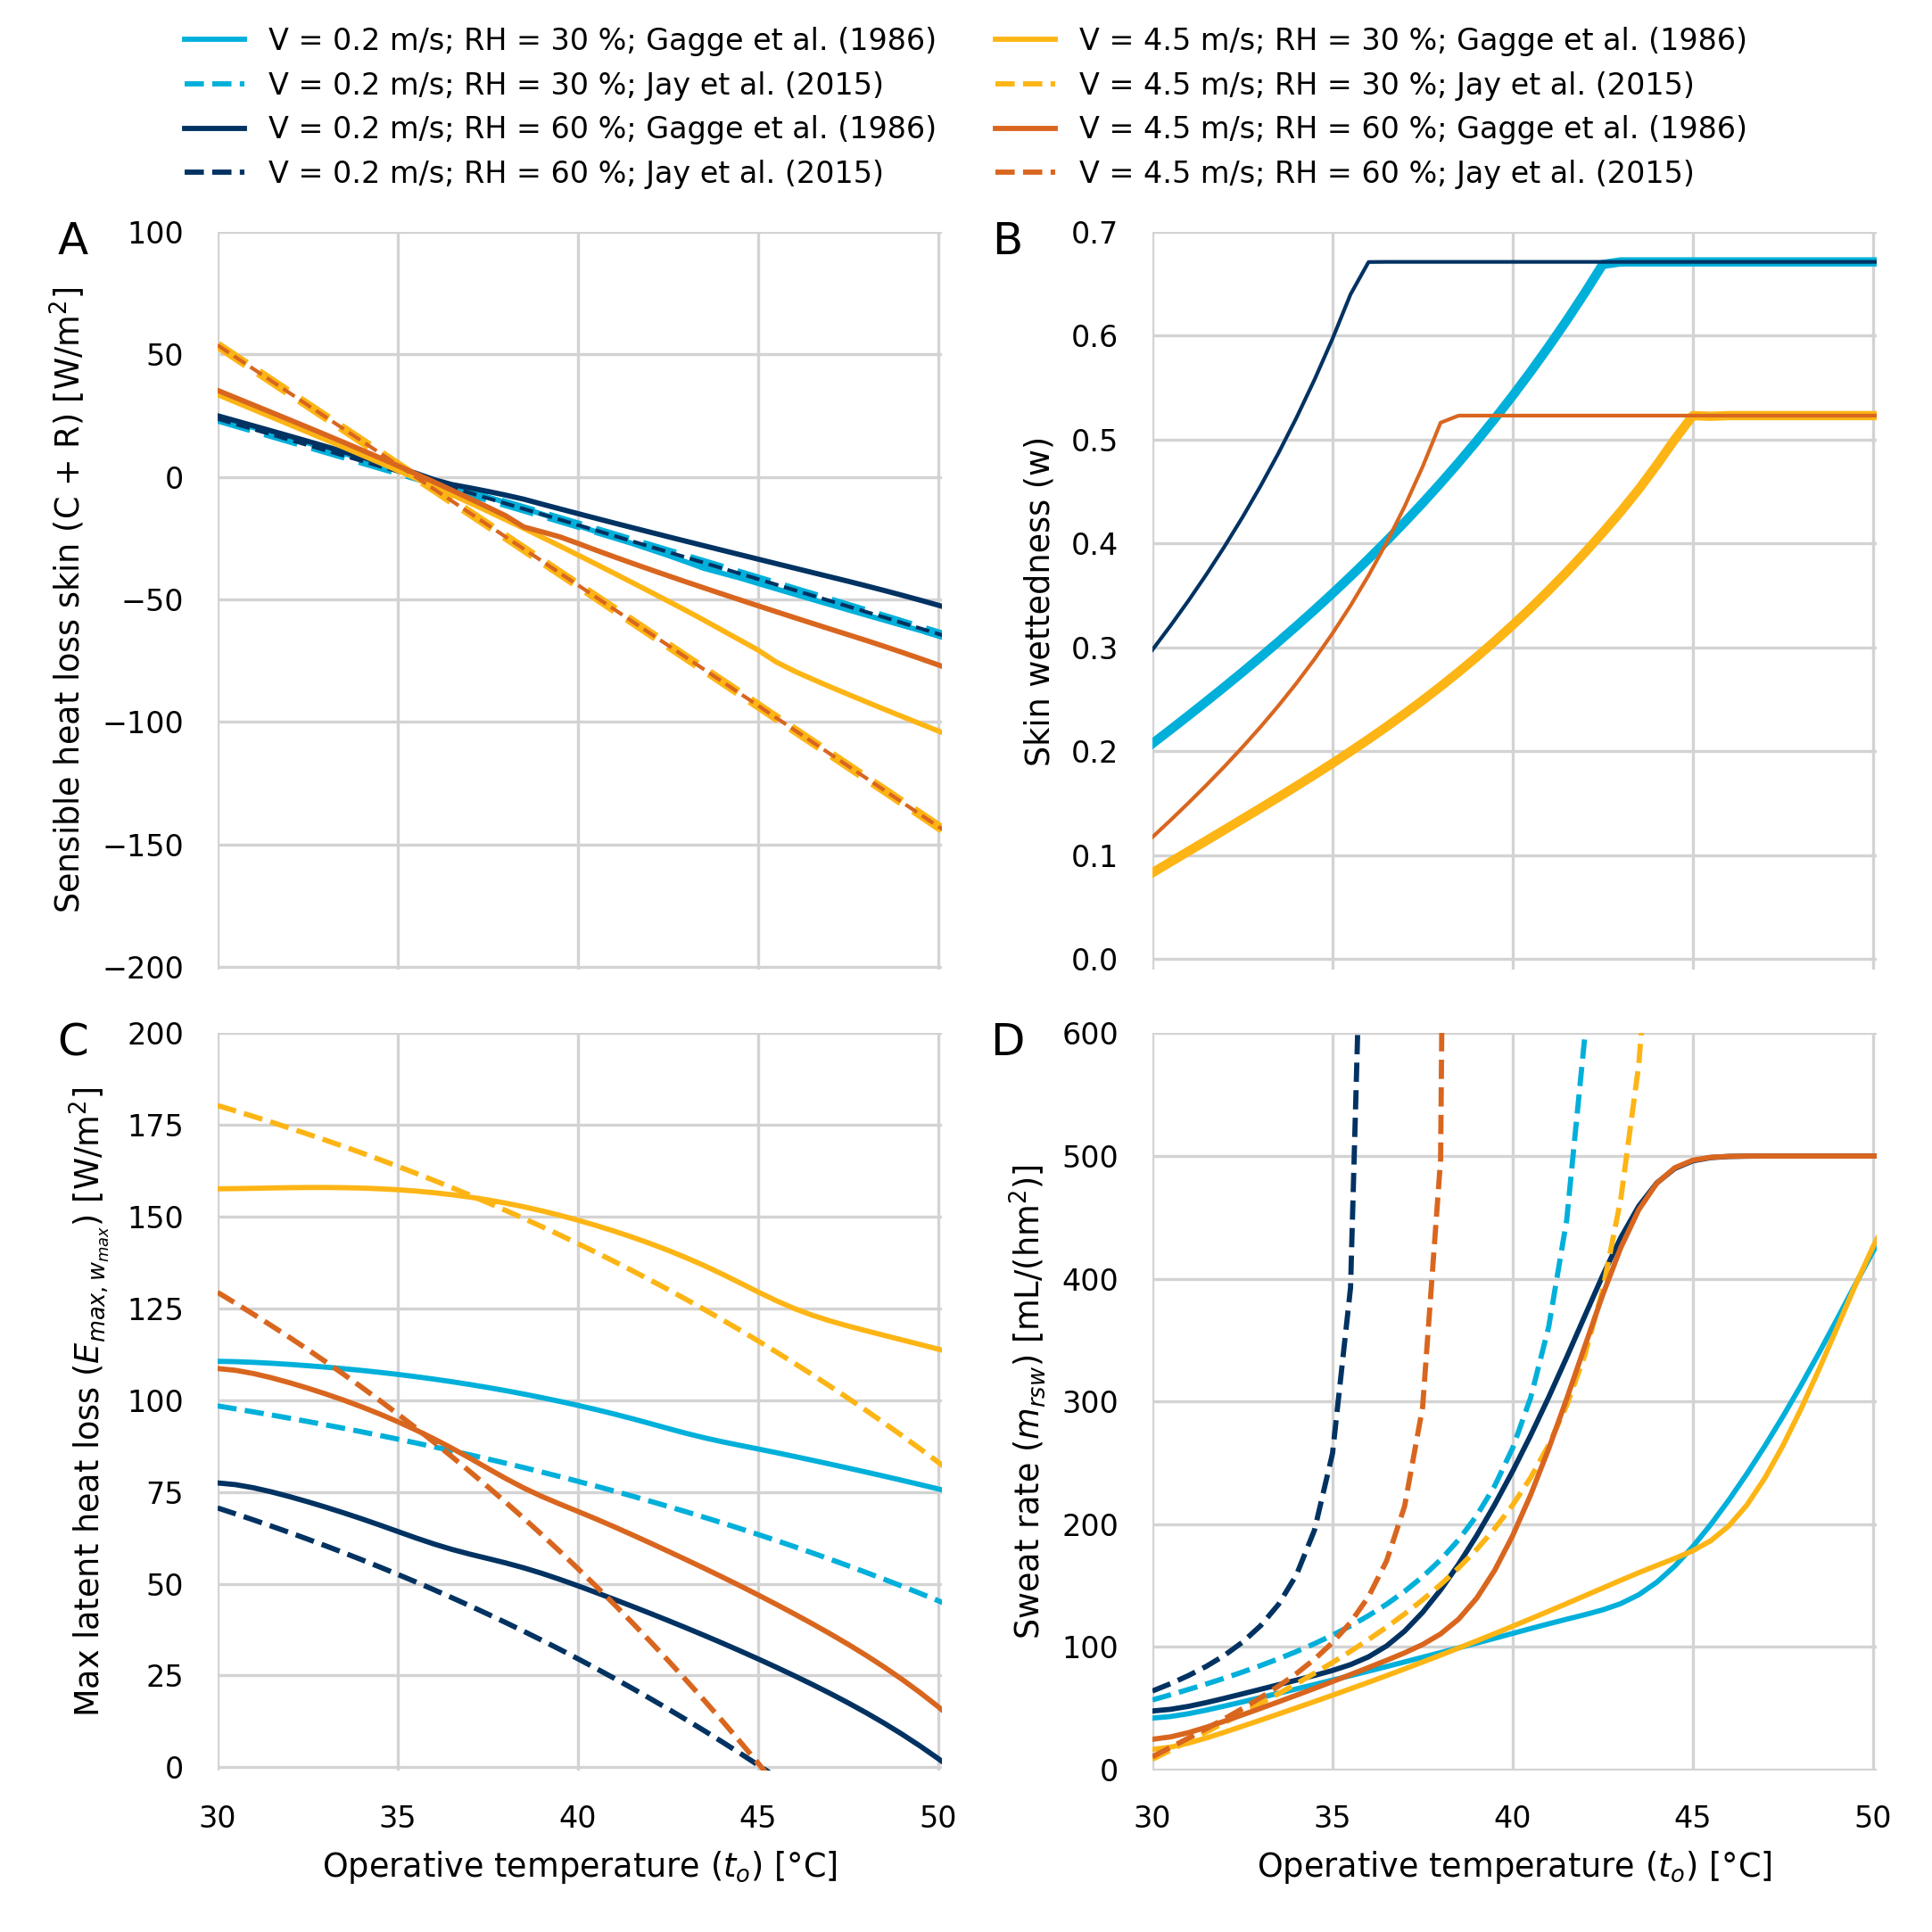
\includegraphics[width=\textwidth]{figures/comparison_models_v2}
    \caption{Results obtained with the energy models proposed by \mycite{Jay2015} and \mycite{GaggeSET}.
    Each Figure shows how a variable changes as a function of \ac{t-op} for a set combination of \ac{rh} and \ac{v}.
    Figure: A) \Acf{c-r}.
    B) \Acf{w}.
    C) \Acf{e-max} estimated using \ac{w} = \ac{w-max}.
    D) \Acf{m-sweat}.}
    \label{fig:comparison_models}
\end{figure*}

The former model iteratively determines \ac{t-sk}, while the latter assumes it to be constant and equal to 35~$^{\circ}$C\@, which is equivalent to a fully vasodilated state.
When heat gains exceed heat losses, the \mycite{GaggeSET} model estimates that some heat energy is stored in the body and consequently \ac{t-sk} increases, as shown in Figure~\ref{fig:results_model_2}A and ~\ref{fig:results_model_2}C, respectively.
This reduces the rate at which sensible heat gain increases as \ac{t-op} increases.

\begin{figure*}[thb!]
    \centering
    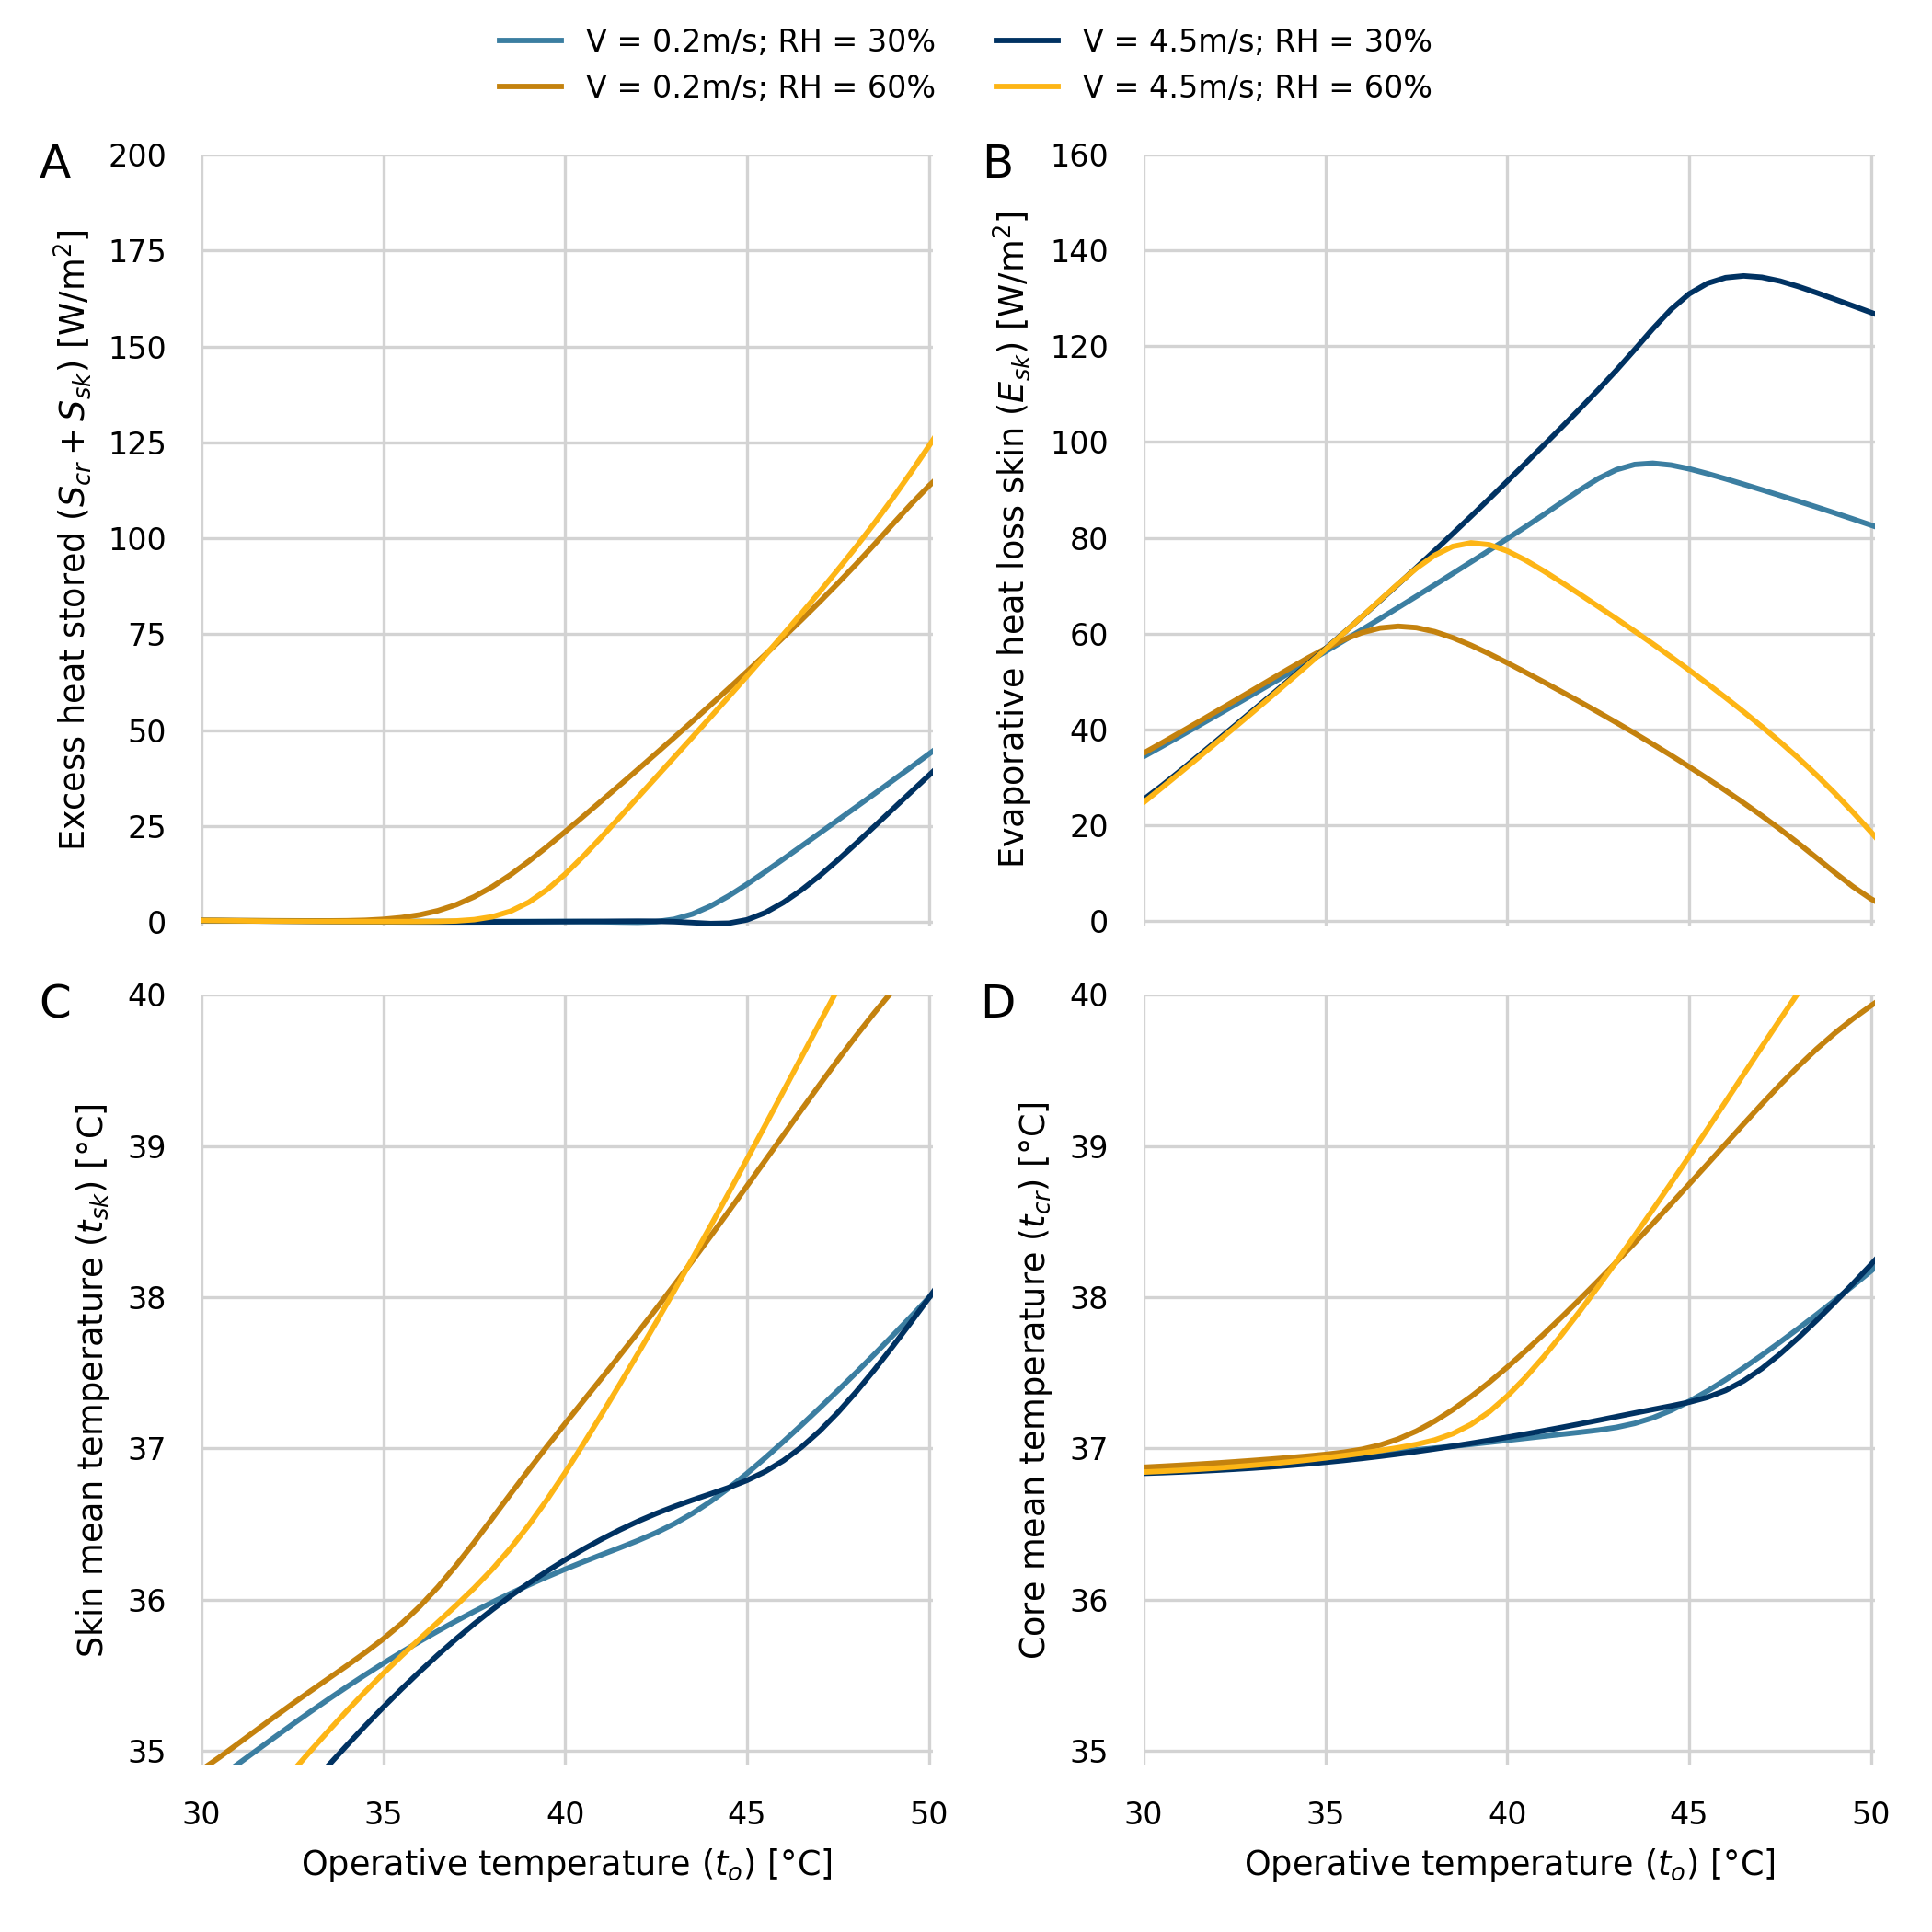
\includegraphics[width=\textwidth]{figures/results_model_2}
    \caption{Results obtained with \mycite{GaggeSET} energy model.
    Each Figure shows how a variable changes as a function of \ac{t-op} for a set combination of \ac{rh} and \ac{v}.
    Figure: A)  Excess heat stored in the human body, skin and core compartments (\ac{s-sk} + \ac{s-cr}).
    B) \Acf{e-sk}.
    C) \Acf{t-sk}.
    D) \Acf{t-cr}.}
    \label{fig:results_model_2}
\end{figure*}

The values of \ac{w} for two air speeds are shown in Figure~\ref{fig:comparison_models}B\@.
The skin wettedness is allowed by the model to increase until it reaches the value of \ac{w-max}, after that, it plateaus and remains constant and thermal stress is expected to occur.
For young adults, \mycite{Jay2015} assumed \ac{w-max} to be equal to 0.65 for the `fan on' condition and 0.85 for the `fan off' condition.
The values of \ac{w-max} estimated by the \mycite{GaggeSET} for the same air speeds are lower (Figure~\ref{fig:comparison_models}B).
% todo SS It is always better to be direct and use the active voice. There are several situations in the paper where the readability can be improved.
The operative temperature at which \ac{w} equals \ac{w-max} is inversely proportional to the value of \ac{rh}.
For \ac{t-op} higher than \ac{t-sk}, the negative effect that an increase in \ac{v} has on sensible heat gain is compensated by a greater increase in the \acf{e-sk} that the body can dissipate towards the surrounding environment.
For example, when \ac{t-op}~=~45~$^{\circ}$C and \ac{rh}~=~30~\%, a change in \ac{v} from 0.2 to 4.5~m/s increases (\acs{c-r}) by \var{increase_sensible_v_02_45}~W/m\textsuperscript{2} while increasing \ac{e-sk} by \var{increase_latent_v_02_45}~W/m\textsuperscript{2}, which provides a net positive effect.

Figure~\ref{fig:comparison_models}C shows the values of \ac{e-max} estimated by replacing \ac{w} in Equation~\ref{eq:latent-skin} with \ac{w-max}.
The value of \ac{e-max} decreases as \ac{t-op} increases since \ac{p-a} grows more rapidly than \ac{p-sk}.
For a set combination of \ac{v} and \ac{t-op} the value of \ac{e-max} decreases as the value of \ac{rh} increases because humid air has a higher \ac{p-a} than dry air.
The reduction in \ac{e-max} estimated by \mycite{GaggeSET} model is lower than the one estimated by \mycite{Jay2015} since an increase in \ac{t-sk} elevates the vapor pressure gradient between the skin and its surrounding environment.

The \acf{m-sweat} is shown in Figure~\ref{fig:comparison_models}D\@.
The difference between the results obtained with the two heat balance models can be attributed to the fact that \citeauthor{Jay2015} calculate the value of \ac{m-sweat} as a function of the required latent energy that the body should, in theory, dissipate to achieve thermal neutrality and the required evaporative efficiency of sweating (i.e., the amount of sweat produced that evaporates).
The latter was estimated using ISO 7933 equation and it is estimated as a function of \ac{w} alone.
On the other hand, \citeauthor{GaggeSET} calculate the value of \ac{m-sweat} as a function of regulatory signals and they assume that \ac{m-sweat} cannot exceed 500~mL/h.

% todo Ollie Jay: I think that when the Gagge model reaches a steady-state the sweat output should be the same as that required to achieve Ereq (adjusted for differences in sweating efficiency). I am pretty sure that is the basis of the PHS as well - in fact I think the PHS' predecessor, which the PHS built upon,  was called the required sweat rate for heat balance index

The excess heat stored in the human body (\acs{s-cr} + \acs{s-sk}), \ac{t-sk}, and \ac{t-cr} are shown in Figure~\ref{fig:results_model_2}A, \ref{fig:results_model_2}C, and \ref{fig:results_model_2}D, respectively.
When the body can no longer dissipate exogenous and endogenous heat gains, the excess heat causes \ac{t-sk} and \ac{t-cr} to rise.

\subsection{Heat Stress}\label{subsec:heat-stress}

The combination of \ac{t-op}, \ac{rh}, and \ac{v} at which heat stress is predicted to occur is presented in Figure~\ref{fig:comparison_air_speed}.

\begin{figure}[thb!]
    \centering
    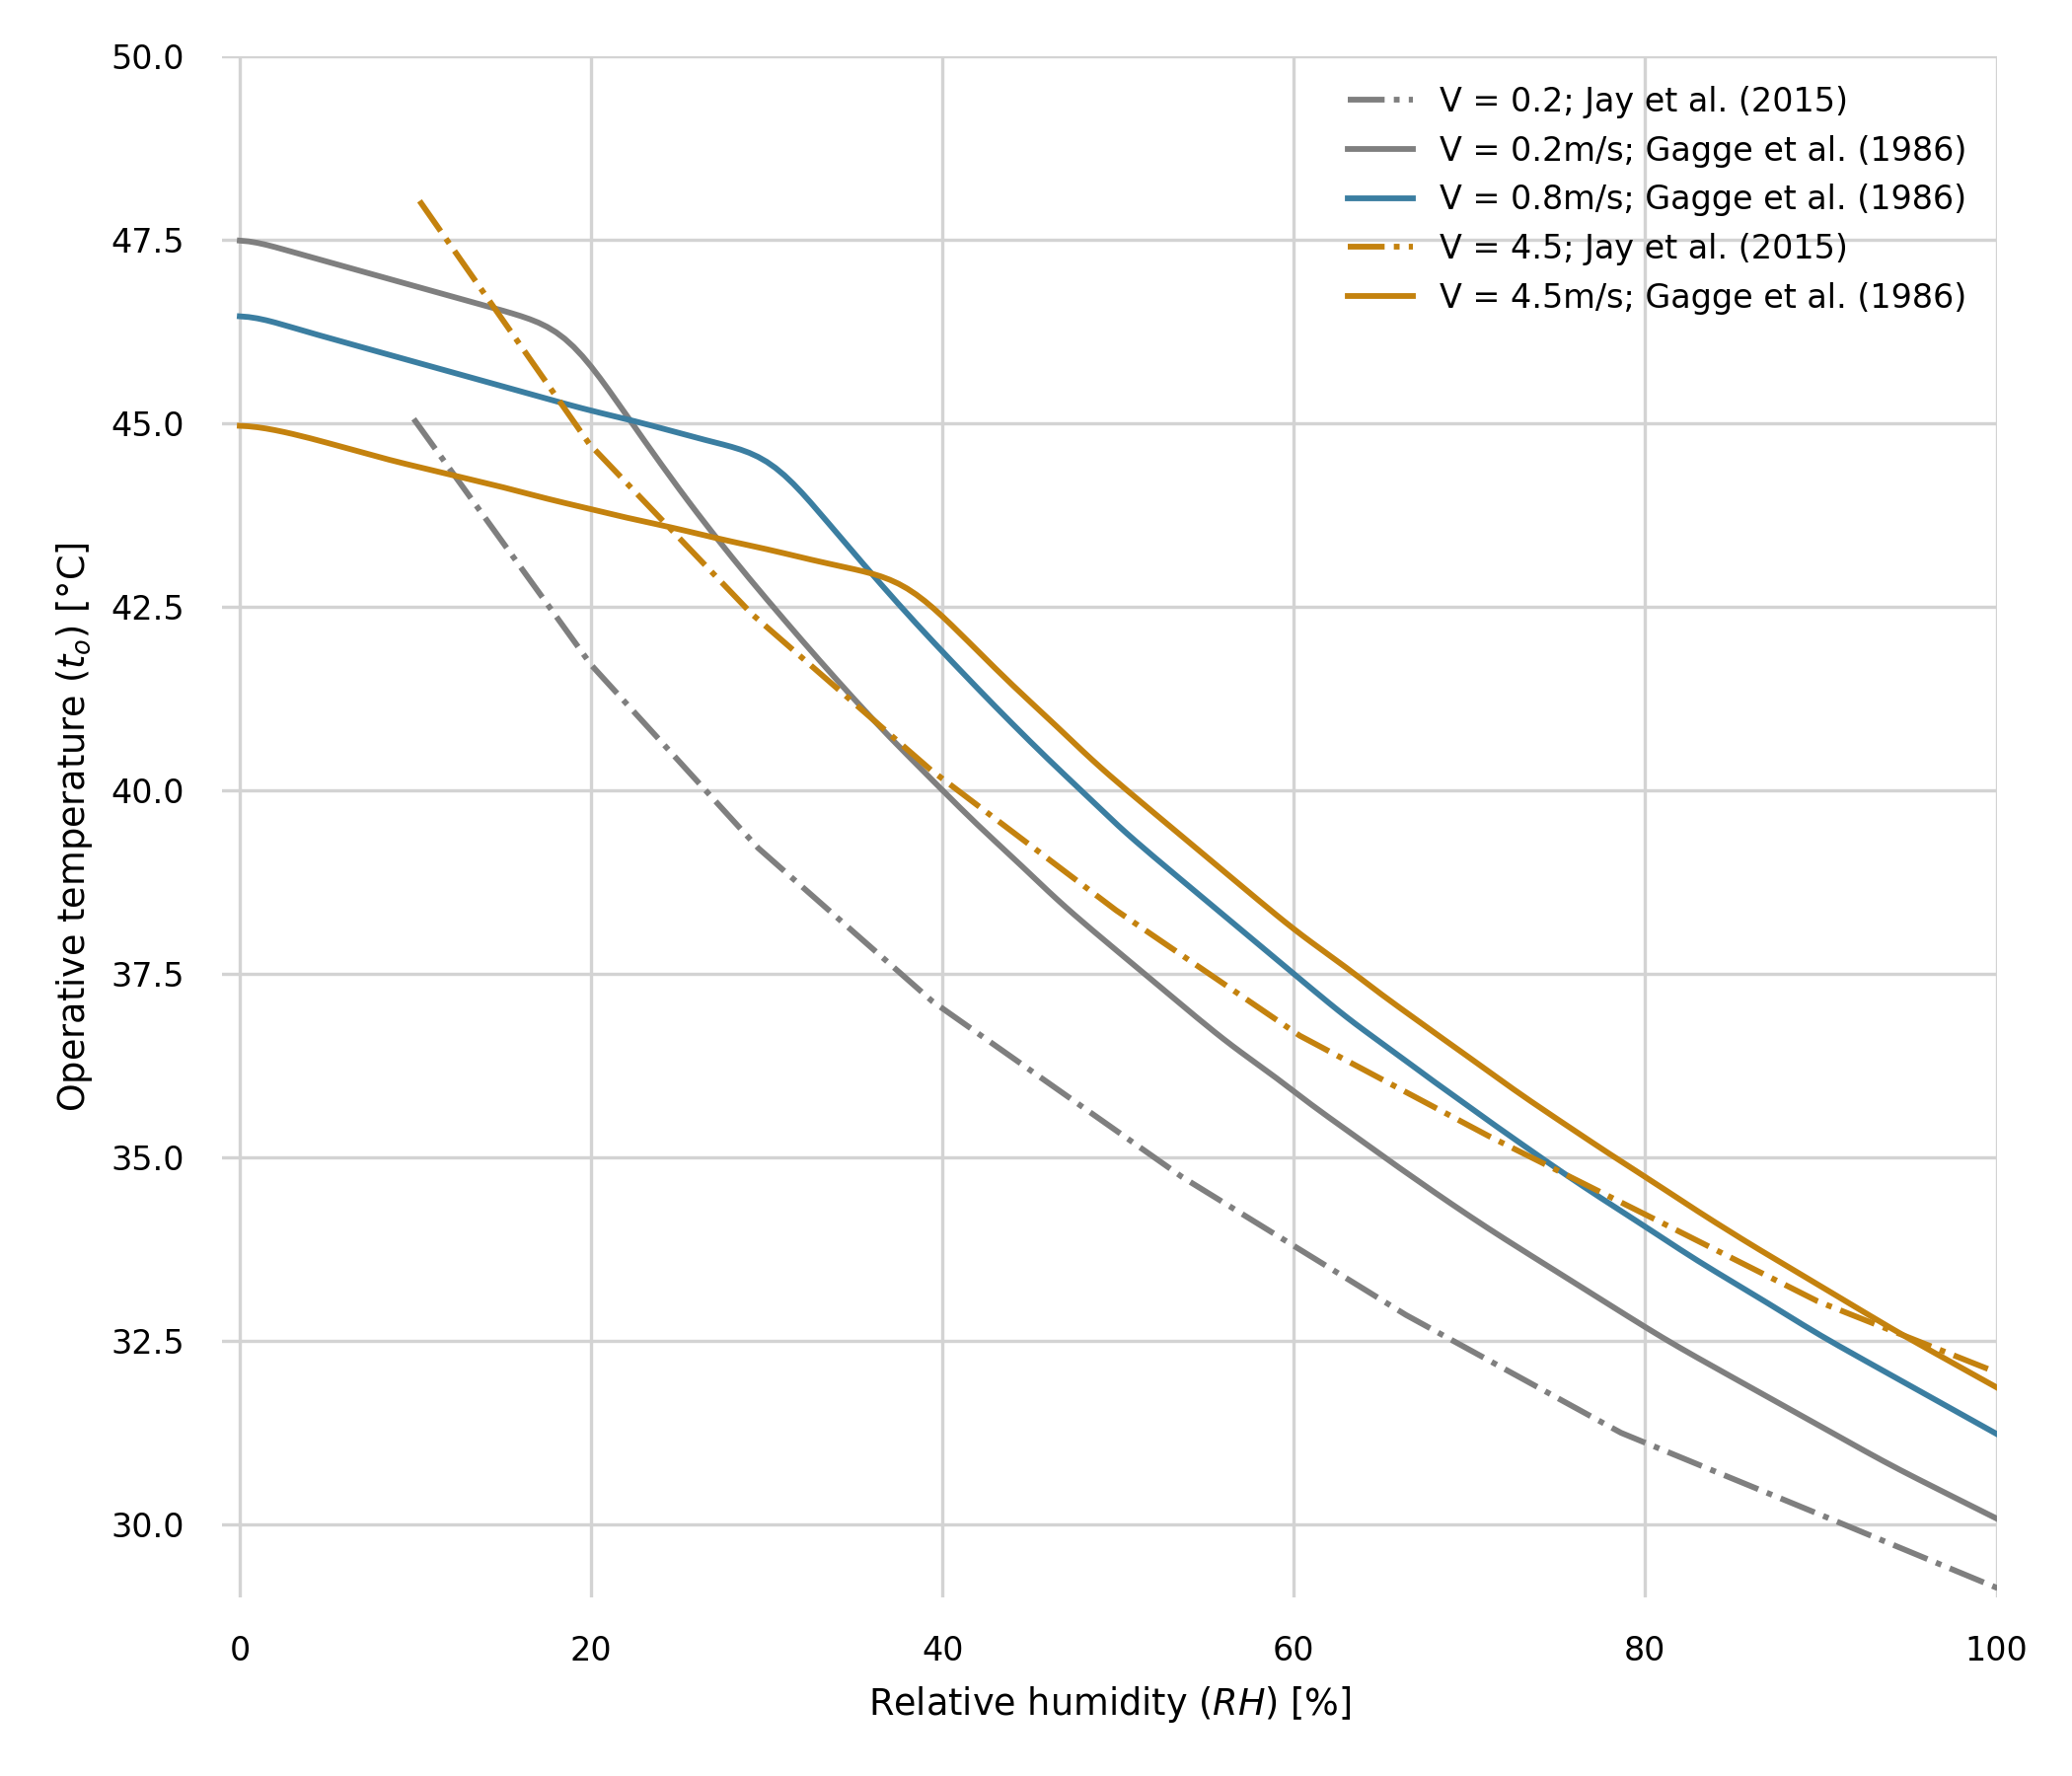
\includegraphics[width=0.5\textwidth]{figures/comparison_air_speed}
    \caption{Predicted limits above which thermal strain is estimated to occur.
    The figure shows the results calculated using the \mycite{GaggeSET} model and the \mycite{Jay2015} models.
    Each line demarcates the point above which heat strain is expected to occur.}
    \label{fig:comparison_air_speed}
\end{figure}

Each line demarcates the conditions above which not all adult healthy individuals would be able to compensate for endogenous and exogenous heat gains and therefore, if possible, they should avoid being exposed to these conditions.
The Figure shows the results obtained with both the \mycite{GaggeSET} and the \mycite{Jay2015} models.
For a specific value of \ac{v}, the maximum \ac{t-op} at which heat strain is estimated to occur decreases as the value of \ac{rh} increases since, as previously shown, the value of \ac{e-max} is inversely proportional to \ac{rh}.
In addition, for a specific value of \ac{rh}, as the value of \ac{v} grows, the overall increase in the maximum critical temperature rapidly decreases, this is not show in the Figure.
For example, in an environment with \ac{rh}~=~60~\%, increasing \ac{v} from 0.2~m/s to 0.8~m/s and then to 4.5~m/s leads to an increase of the critical temperature of approximately \var{increase_t_strain_v_08}~$^{\circ}$C and \var{increase_t_strain_v_45}~$^{\circ}$C, respectively.
The slope of the heat stress curve flattens at low values of \ac{rh}.
The \ac{rh} value at which the curve flattens is proportional to \ac{v}.
This can be explained by the fact (not shown in the Figures) that for low values of \ac{rh} skin blood flow reaches its upper limit causing thermal strain.
Consequently, in the region where the heat stress curve for elevated air speeds is lower than the one for `still air' electric fans should not be used, unless the hot and dry air is pre-cooled to a point below the `elevated air speed' heat stress line.
This can be achieved using passive cooling strategies such as evaporative cooling.
\mycite{Jay2015} model fails to account for this aspect and overestimates the benefits of using fans for \ac{rh} values lower than 20~\% and \ac{t-db} above 46~$^{\circ}$C, please refer to Section~\ref{subsec:model-validation-experimental-data} for more information.

% todo Ollie Jay: I actually think the overestimation of the efficacy of fan use with our old model occurs at much lower temperatures.. Based on all of the physiological data I am concerned that the present model overestimates the beneifits of fan use at these very dry and hot temperatures. I think that if we assessed fan use at say 42 or 43C and 5%RH, fans would be detrimental even in healthy young people

\subsection{Metabolic Rate and Clothing}\label{subsec:met-clo}

To better understand how personal factors would impact the body's ability to dissipate heat, we calculated when heat stress would occur for different combinations of \ac{met} and \ac{clo}.
Results for people wearing light summer clothing (walking shorts, short-sleeve shirt and sandals, \acs{clo}~=~0.36~clo), and office summer clothing (trousers, short-sleeve shirt, and closed shoes \acs{clo}~=~0.5~clo) who are either seated reading or writing (\ac{met}~=~1.0 met) or standing relaxed (\ac{met}~=~1.2~met) are shown in Figure~\ref{fig:met_clo}.

\begin{figure}[thb!]
    \centering
    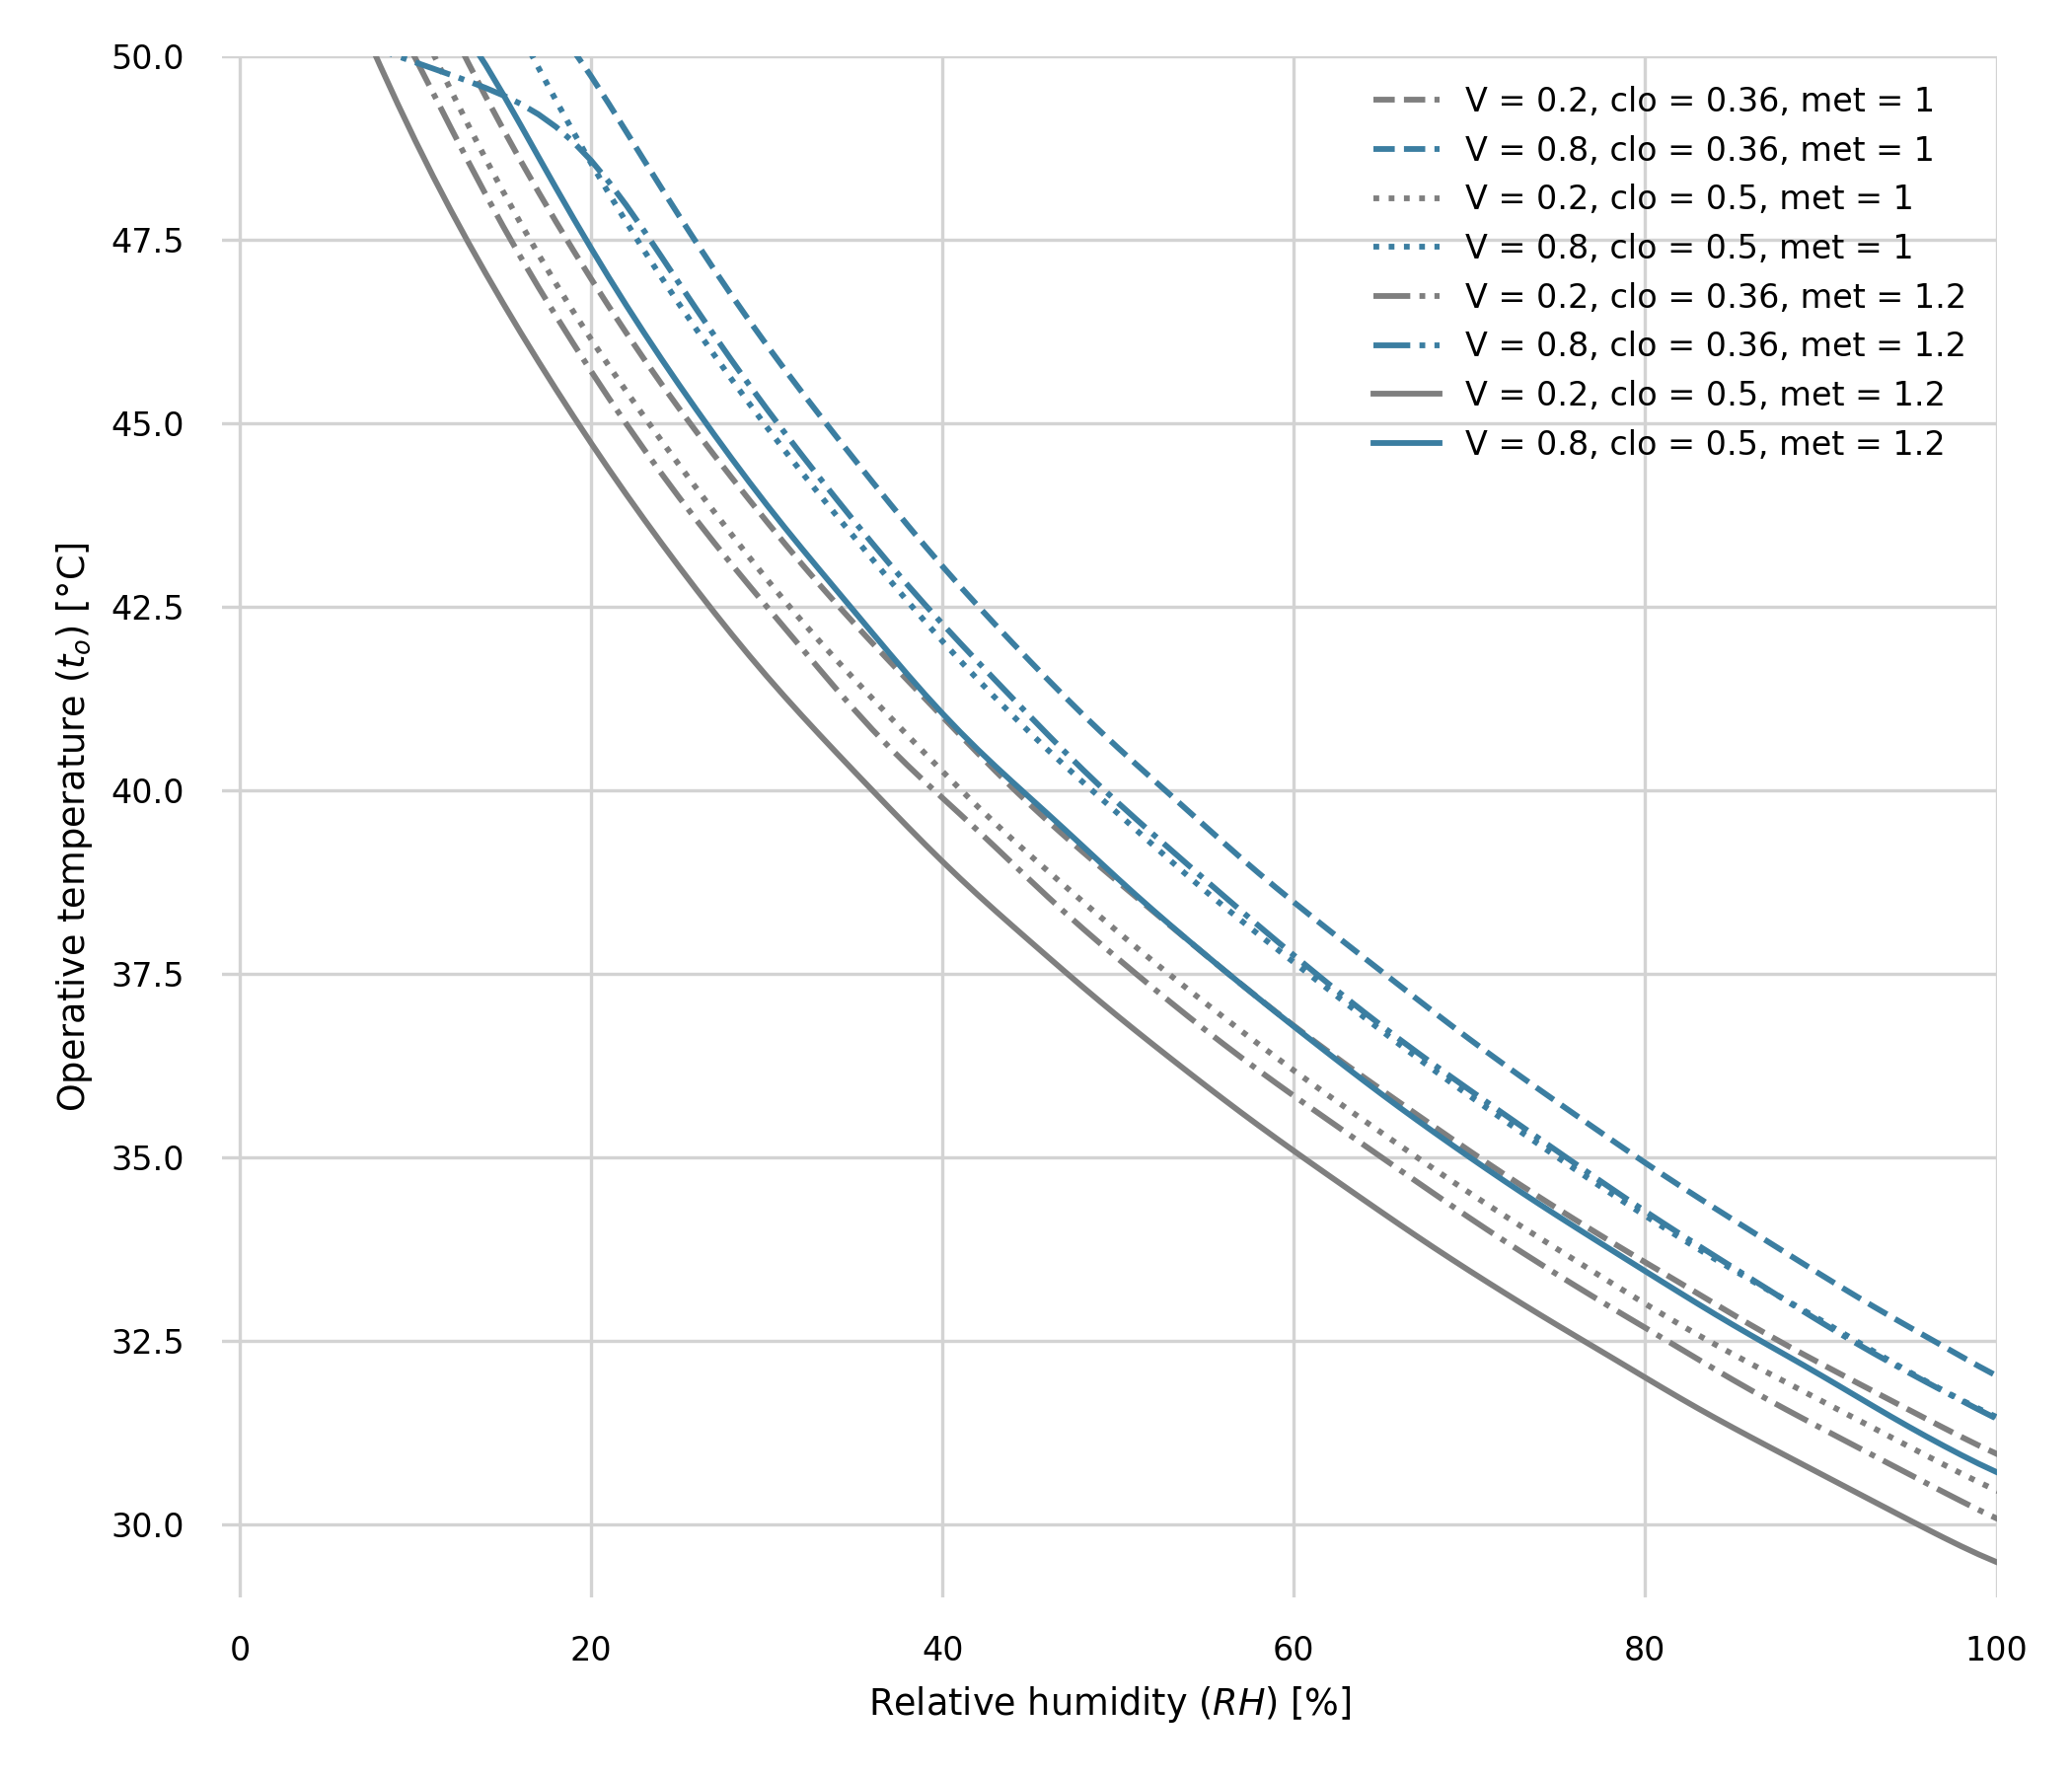
\includegraphics[width=0.5\textwidth]{figures/met_clo}
    \caption{Each line demarcates how different combinations of personal factors (e.g., \ac{met}, \ac{clo}) and environmental factors affect the point above which the body cannot longer dissipate all the endogenous and exogenous heat gains.}
    \label{fig:met_clo}
\end{figure}

As expected, decreasing both \ac{met} and \ac{clo} has a net positive effect since it reduces both heat gain and thermal resistance, respectively.
For values of \ac{rh} below 20~\% the model predicts that heat strain will be delayed by slightly increasing clothing levels.
In these conditions people can easily sweat despite the higher clo level and additional clothing will reduce sensible heat gains.
It should, however, be noted that these results are affected by \ac{i-cl}.

% todo huizenga: Do you want to mention vapor permeability of clothing here or is that too much detail?

\subsection{Model Validation Using Experimental Data}\label{subsec:model-validation-experimental-data}

To validate the results obtained with the \mycite{GaggeSET} model, we examined how the predicted value of \ac{t-cr} varies as a function of \ac{rh}, under a set of specific conditions as tested experimentally by \mycite{Rate2015} (e.g., \ac{t-db}~=~42~$^{\circ}$C, \ac{v}~=~4.0~m/s, \ac{clo}~=~0.35~clo, and \ac{met}~=~1.0~met).
The results are shown in Figure~\ref{fig:comparison_ravanelli}.
It should be noted that \mycite{Rate2015} only reported the core body temperature of one participant.
% todo compare with the full dataset
Consequently, despite the agreement with their experimental data (mean absolute error~=~\var{mean_abs_err_ravanelli}~$^{\circ}$C), more experimental data is needed for validation.
% todo SS From this text it seems that the ONLY validation for the gagge model is this comparison with one subject that you did. Are you sure about this? I guess that there are papers out there that verified if Gagge model was accurate to predict core temperature. Given that you are not giving a real validation, maybe it is better to reference to more extensive valudations and remove this part. If this is the only validation, then consider moving it as appendix.

% todo Ollie Jay: I agree with this comment... This one participant was an example and we have the data for the other participants , but still, it is only small subset of individuals so probably does not constitute a validation.

\begin{figure}[thb!]
    % todo check font size
    \centering
    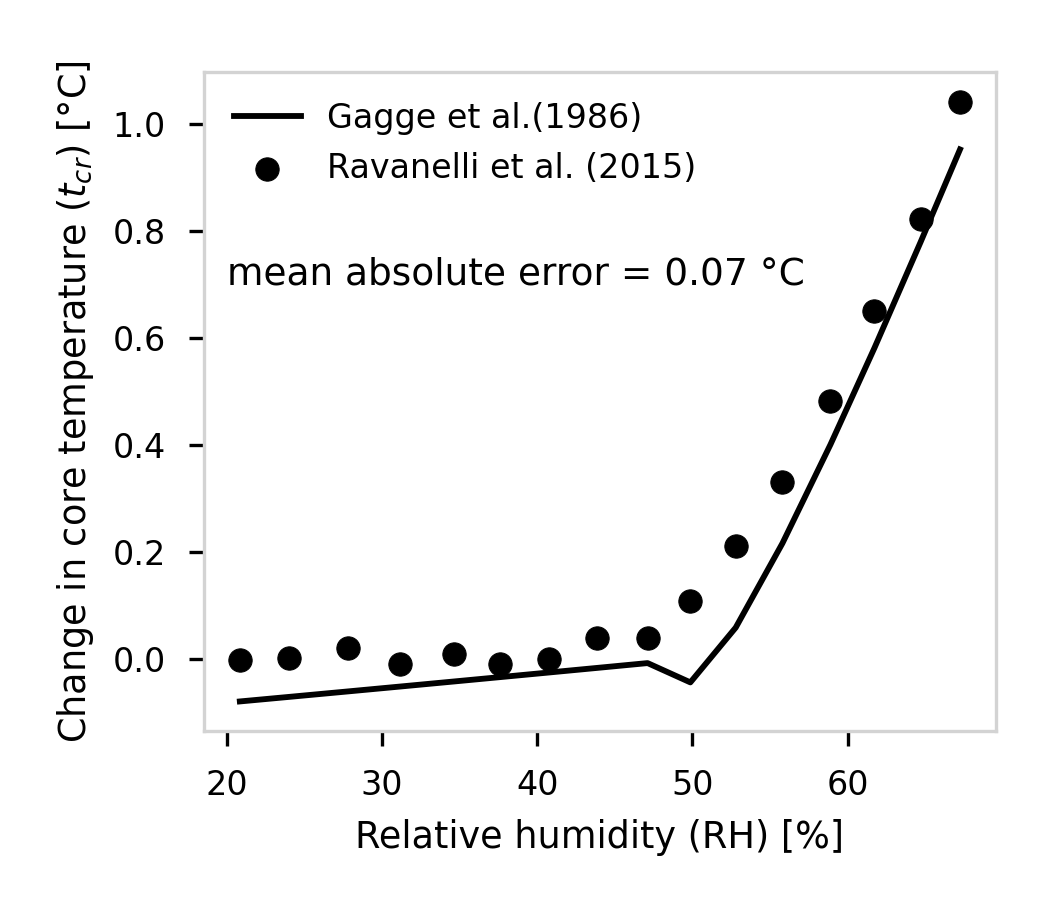
\includegraphics[width=0.5\textwidth]{figures/comparison_ravanelli}
    \caption{Change in \acf{t-cr} as a function of \acf{rh}.
    Where \ac{t-db}~=~42~$^{\circ}$C, \ac{v}~=~4.0~m/s, \ac{clo}~=~0.35~clo, and \ac{met}~=~1.0~met.
    The figure shows the results calculated using the \mycite{GaggeSET} model and those obtained experimentally by \mycite{Rate2015}.}
    \label{fig:comparison_ravanelli}
\end{figure}

The environmental conditions above which the use of elevated air speeds would be detrimental according to \mycite{GaggeSET} model are shown in Figure~\ref{fig:use_fans_experimental}.

\begin{figure*}[thb!]
    \centering
    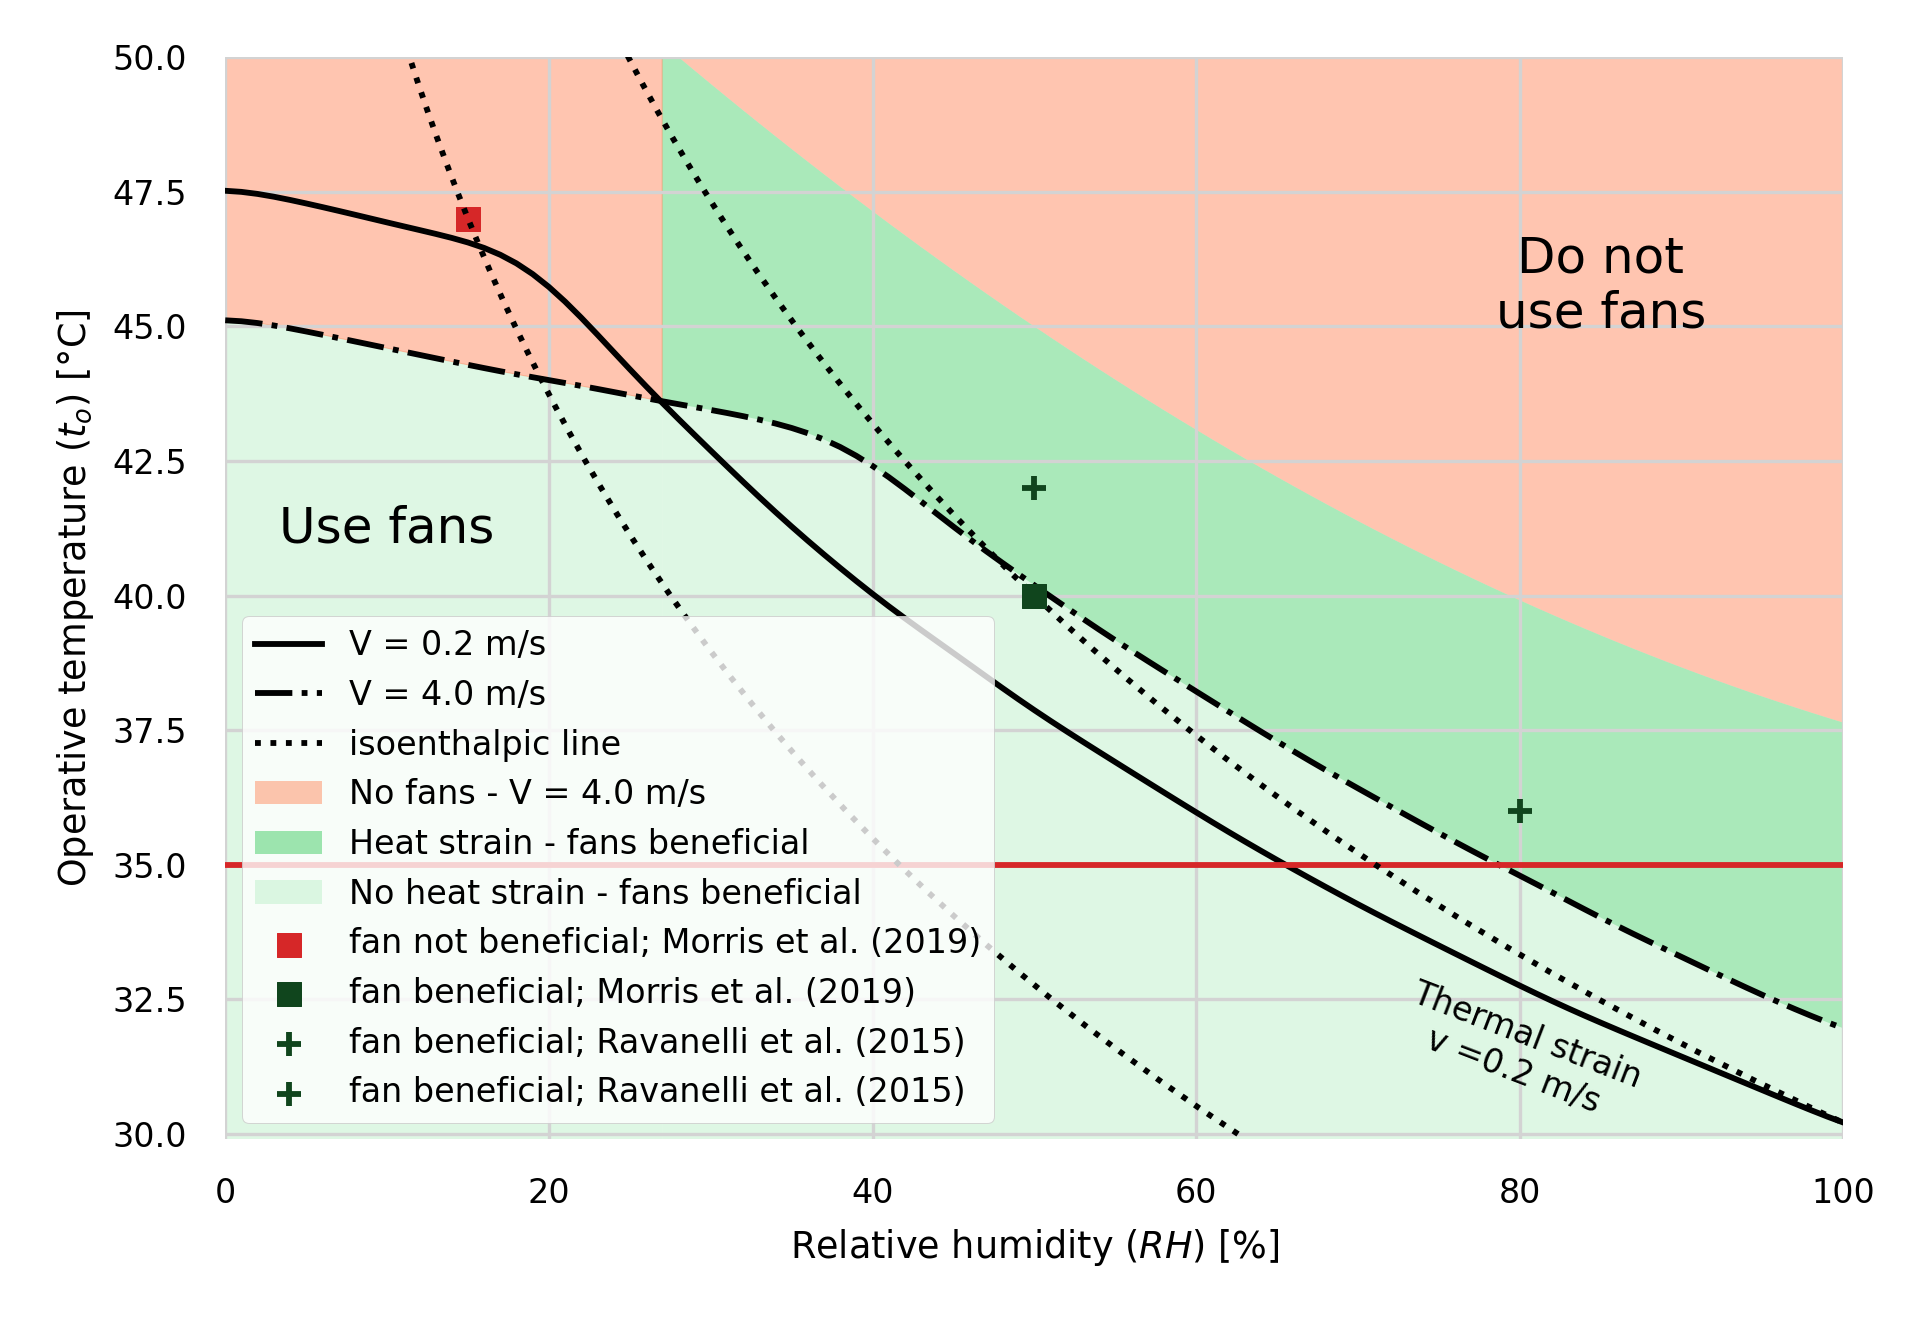
\includegraphics[width=\textwidth]{figures/summary_use_fans_comparison_experimental}
    \caption{The green area shows the environmental conditions in which the use of fans is beneficial since they provide additional cooling to the human body.
    % todo Ollie Jay: I am still uncomfortable with the notion that fans should be recommended up to 45C and 0-5%RH. I do not think this matches the physiological data.
    In the dark green region, while the use of fans is still beneficial, people are most likely to suffer from heat strain.
    The red area demarcates the region in which electric fans should not be used.
    The dotted lines show the isoenthalpic lines passing through the conditions studied by \mycite{Morris2019}.
    We plotted these lines to show that some points in the `do not use fans` region have a lower enthalpy than points in the green area, consequently passive cooling strategies, such as evaporative cooling, may be used to reduce \ac{t-db} to a value within the green region.
    }
    \label{fig:use_fans_experimental}
\end{figure*}

We used a red shading to highlight the region in which electric fans should not be used, while we used a green background to depict when elevated air speed can be used to cool the human body.
We also plotted the lines above which thermal stress is expected to occur (see Figure~\ref{fig:comparison_air_speed} for more details).
As previously mentioned in Section~\ref{subsec:heat-stress} where the heat stress curve for elevated air speeds is lower than the one for `still air' electric fan should not be used.
 However, as shown in Figure~\ref{fig:use_fans_experimental} the enthalpy in the great majority of this region is equal or lower than the enthalpy of the air in the green region.
 Consequently evaporative cooling can be used to first reduce \ac{t-db} to a value within the green region and subsequently electric fans can be safely used.
 Other cooling strategies, such as active cooling, can also be used to cool the air.
 However, we are emphasising the importance of using evaporative cooling since we are assuming that people who mostly rely on electric fans for cooling may not have access to compressor-based air conditioning.
In the dark green area, while the use of fans is still beneficial, not all adult healthy individuals would be able to compensate for endogenous and exogenous heat gains and may experience heat strain.

To validate \mycite{GaggeSET} model results we used experimental data previously published.
In Figure~\ref{fig:use_fans_experimental} we present the results obtained by \mycite{Morris2019} and \mycite{Rate2015}.
The former determined that electric fans (\ac{v}~=~2.0~m/s) are beneficial when \ac{t-db}~=~40~$^{\circ}$C and \ac{rh}~=~51~\%, but should not be used when \ac{t-db}~=~47~$^{\circ}$C and \ac{rh}~=~15~\%.
\mycite{Rate2015} concluded that electric fans (\ac{v}~=~4.0~m/s) help in preventing heat-related elevation in heart rate and \ac{t-cr} in both of the following conditions \ac{t-db}~=~42~$^{\circ}$C and \ac{rh}~=~50~\%, and \ac{t-db}~=~36~$^{\circ}$C and \ac{rh}~=~80~\%.
Results obtained with the \mycite{GaggeSET} model are in agreement with those obtained by both field experiments.

As previously mentioned before, the enthalpy of the air in \mycite{Morris2019} experiment was lower in the scenario with higher temperature and lower \ac{rh}.
The black dashed lines, in Figure~\ref{fig:use_fans_experimental}, are isoenthalpic lines passing through the conditions studied by \mycite{Morris2019}.
Evaporative cooling technologies could, therefore, be used to reduce the value of \ac{t-db} and avoid heat strain.
Evaporative cooling can be achieved by spraying water in the air or even by placing wet towels near the electric fan.

Finally, we compared the results obtained using the \mycite{GaggeSET} with those obtained using the \ac{phs}~\cite{iso7933} and we present the results in Figure~\ref{fig:gagge_phs}.
Results were obtained by comparing the `still air condition' with \ac{v}~=~0.8~m/s, and the predictions of both models overall are similar.
The \ac{phs} model fails to predict that fans should not be used for \ac{rh} values lower than 20~\% and \ac{t-db} above 46~$^{\circ}$C\@.
On the other hand \ac{phs} results are more conservative for high values of \ac{rh}, with the \ac{phs} model discouraging the use of elevated air speeds for \ac{t-db}~=~37.5~$^{\circ}$C and \ac{rh}~=~90~\%\@.
It should be noted that these latter conditions are extremely rare worldwide.

\begin{figure*}[thb!]
    \centering
    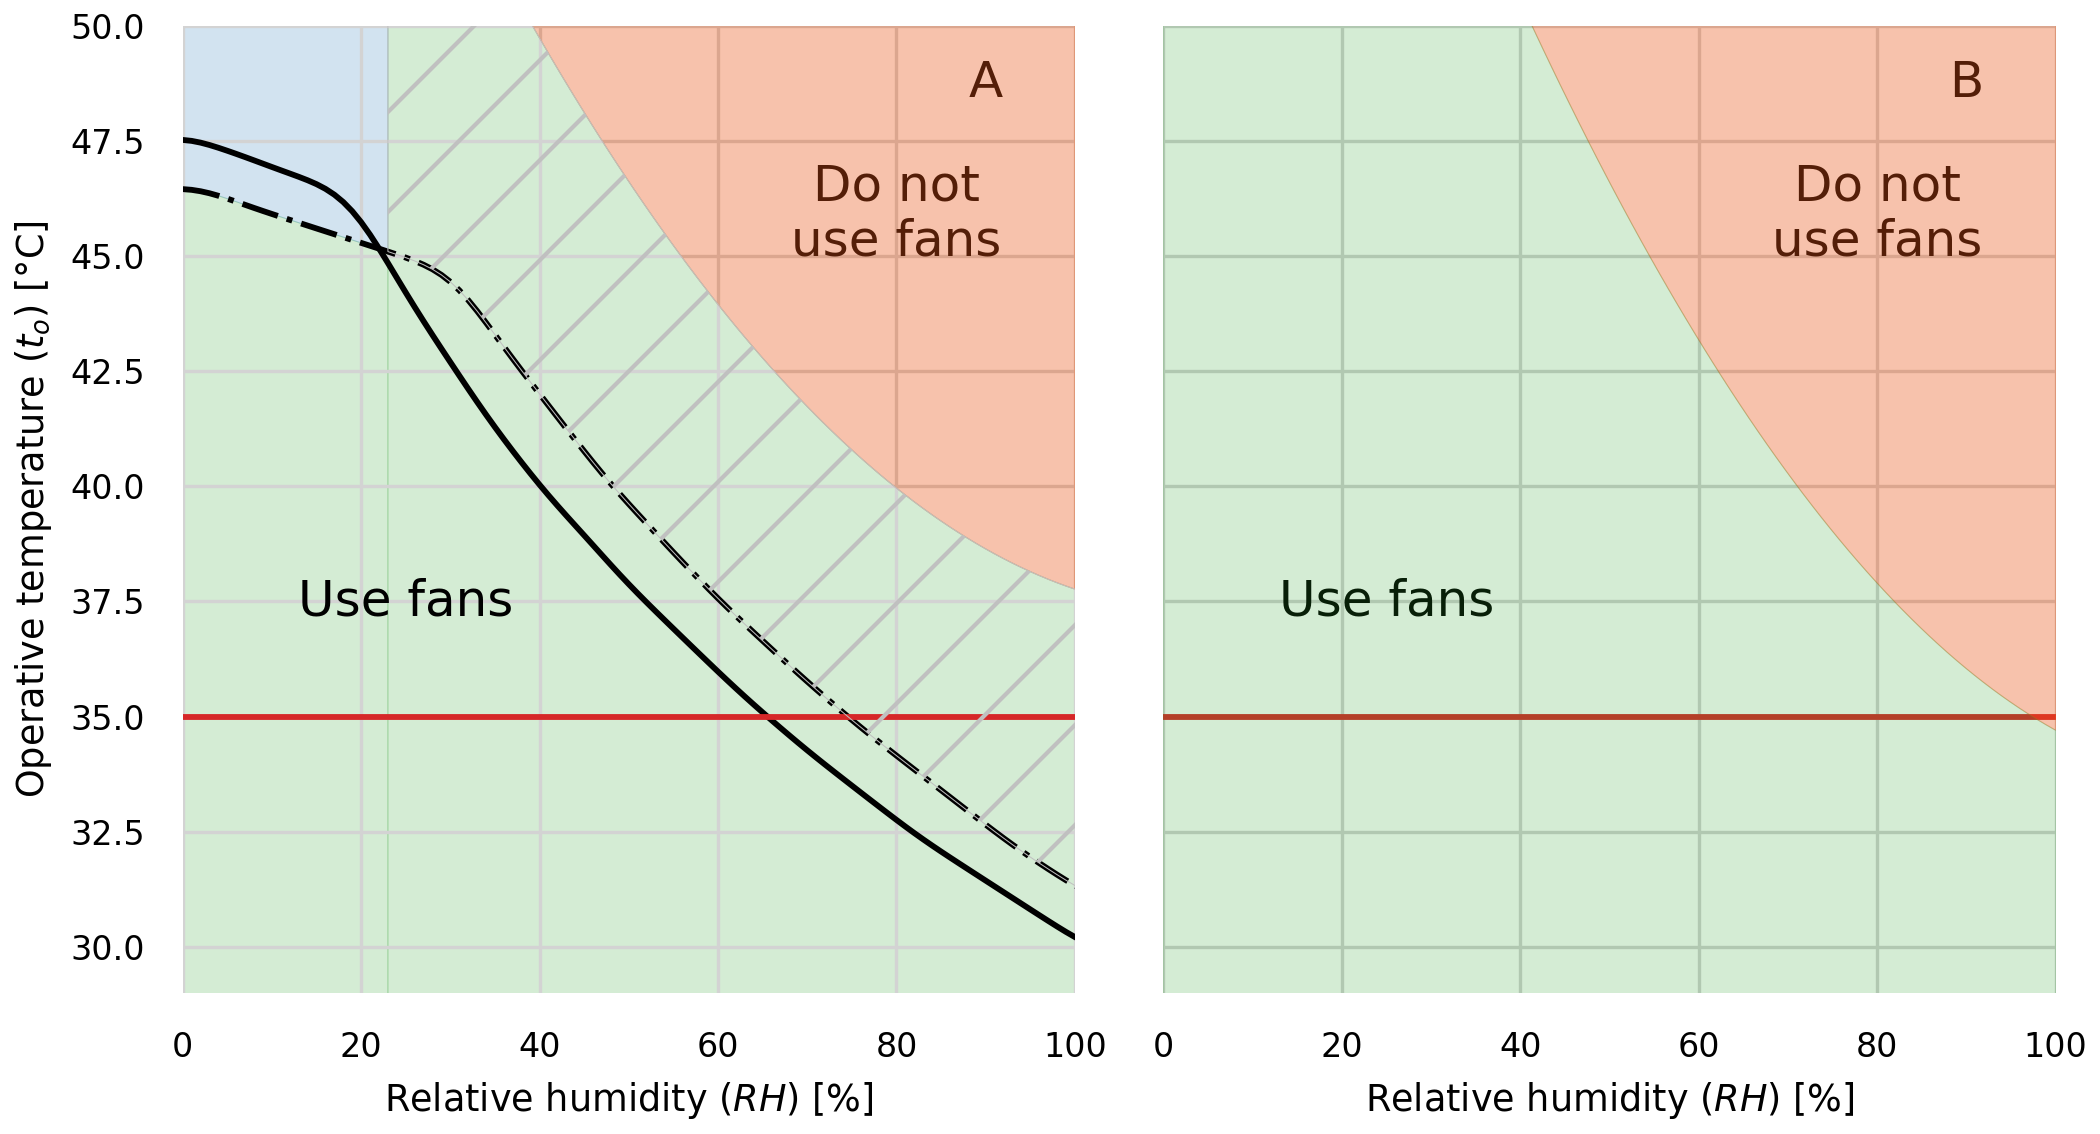
\includegraphics[width=\textwidth]{figures/phs_gagge}
    \caption{Comparison results obtained with \mycite{GaggeSET} (A) and \ac{phs} models (B).
    For more information on how to interpret the Figure please refer to the caption of Figure~\ref{fig:use_fans_experimental}.}
    \label{fig:gagge_phs}
\end{figure*}

\subsection{Benefits of Using Electric Fans}\label{subsec:use-fans}

To understand in which locations worldwide the use of electric fans would be beneficial, in Figure~\ref{fig:energy_storage_delta} we overlaid a plot showing the environmental conditions under which fans can be used with a scatter plot depicting the maximum extreme weather conditions recorded worldwide in more than 5,000 stations.

\begin{figure*}[thb!]
    \centering
    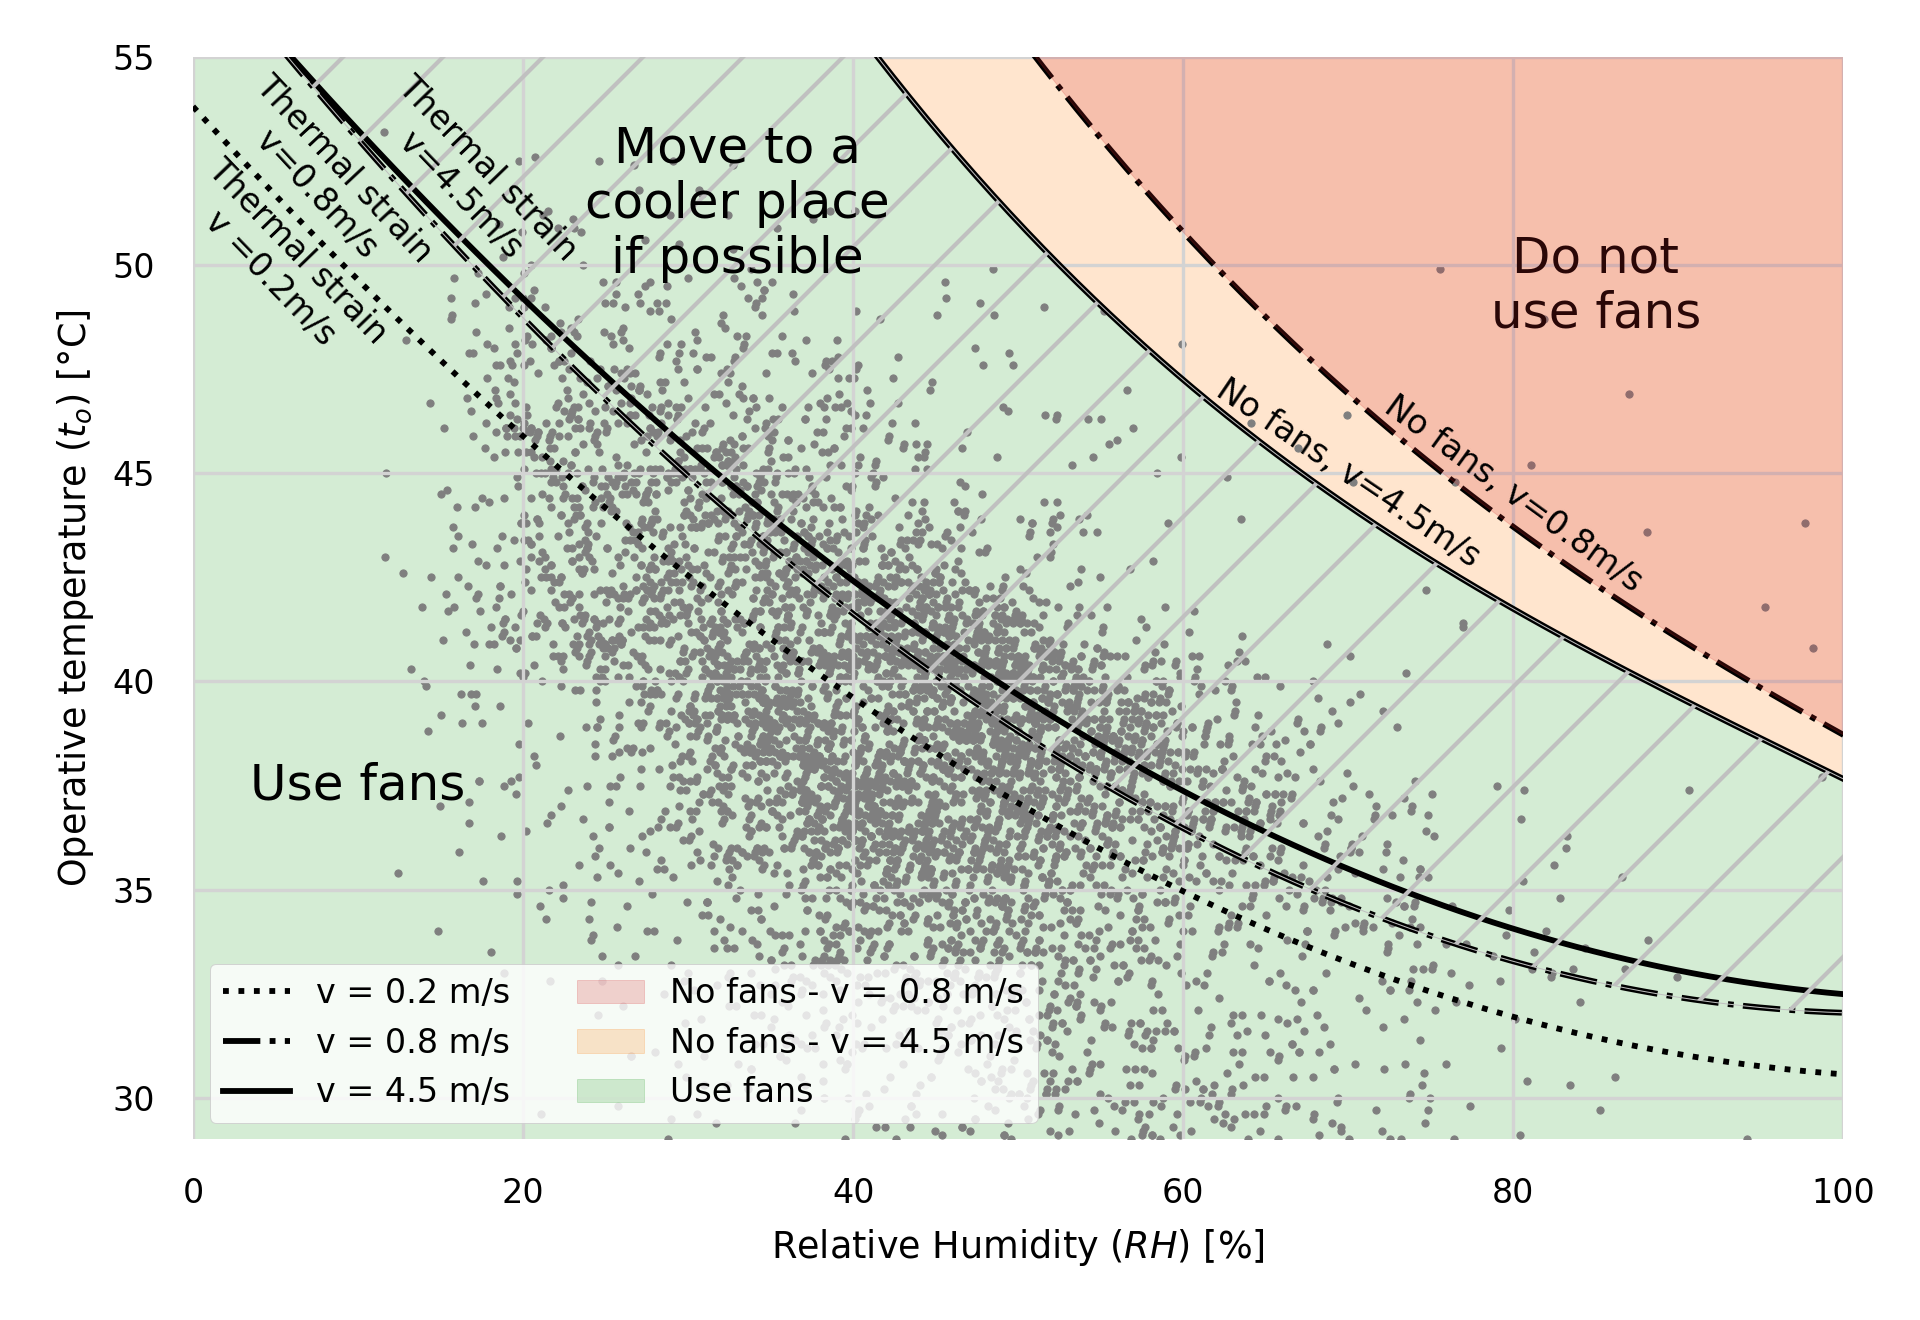
\includegraphics[width=\textwidth]{figures/use_fans}
    \caption{Environmental conditions under which the use of electric fans is beneficial, for more information on how to interpret the Figure please refer to the caption of Figure~\ref{fig:use_fans_experimental}.
    The dots show the maximum extreme climate conditions recorded over the last 20 years in more than 5000 locations worldwide.}
    \label{fig:energy_storage_delta}
\end{figure*}

We determined that in approximately \var{per_location_fans_beneficial_08}~\% of the locations the use of electric fans that can generate \ac{v} up to 0.8~m/s would be beneficial.
In \var{per_location_evaporative_cooling}~\% electric fans should not be used unless any form of cooling (including evaporative cooling) is used to pre-cool the air to any point in the green region.

To better quantify how many people would benefit from the use of electric fans we combined the city with the weather data.
The former contained data from the 115 most populous cities worldwide.
We plotted the data in Figure~\ref{fig:map-population-temperature}.

\begin{figure*}[thb!]
    \centering
    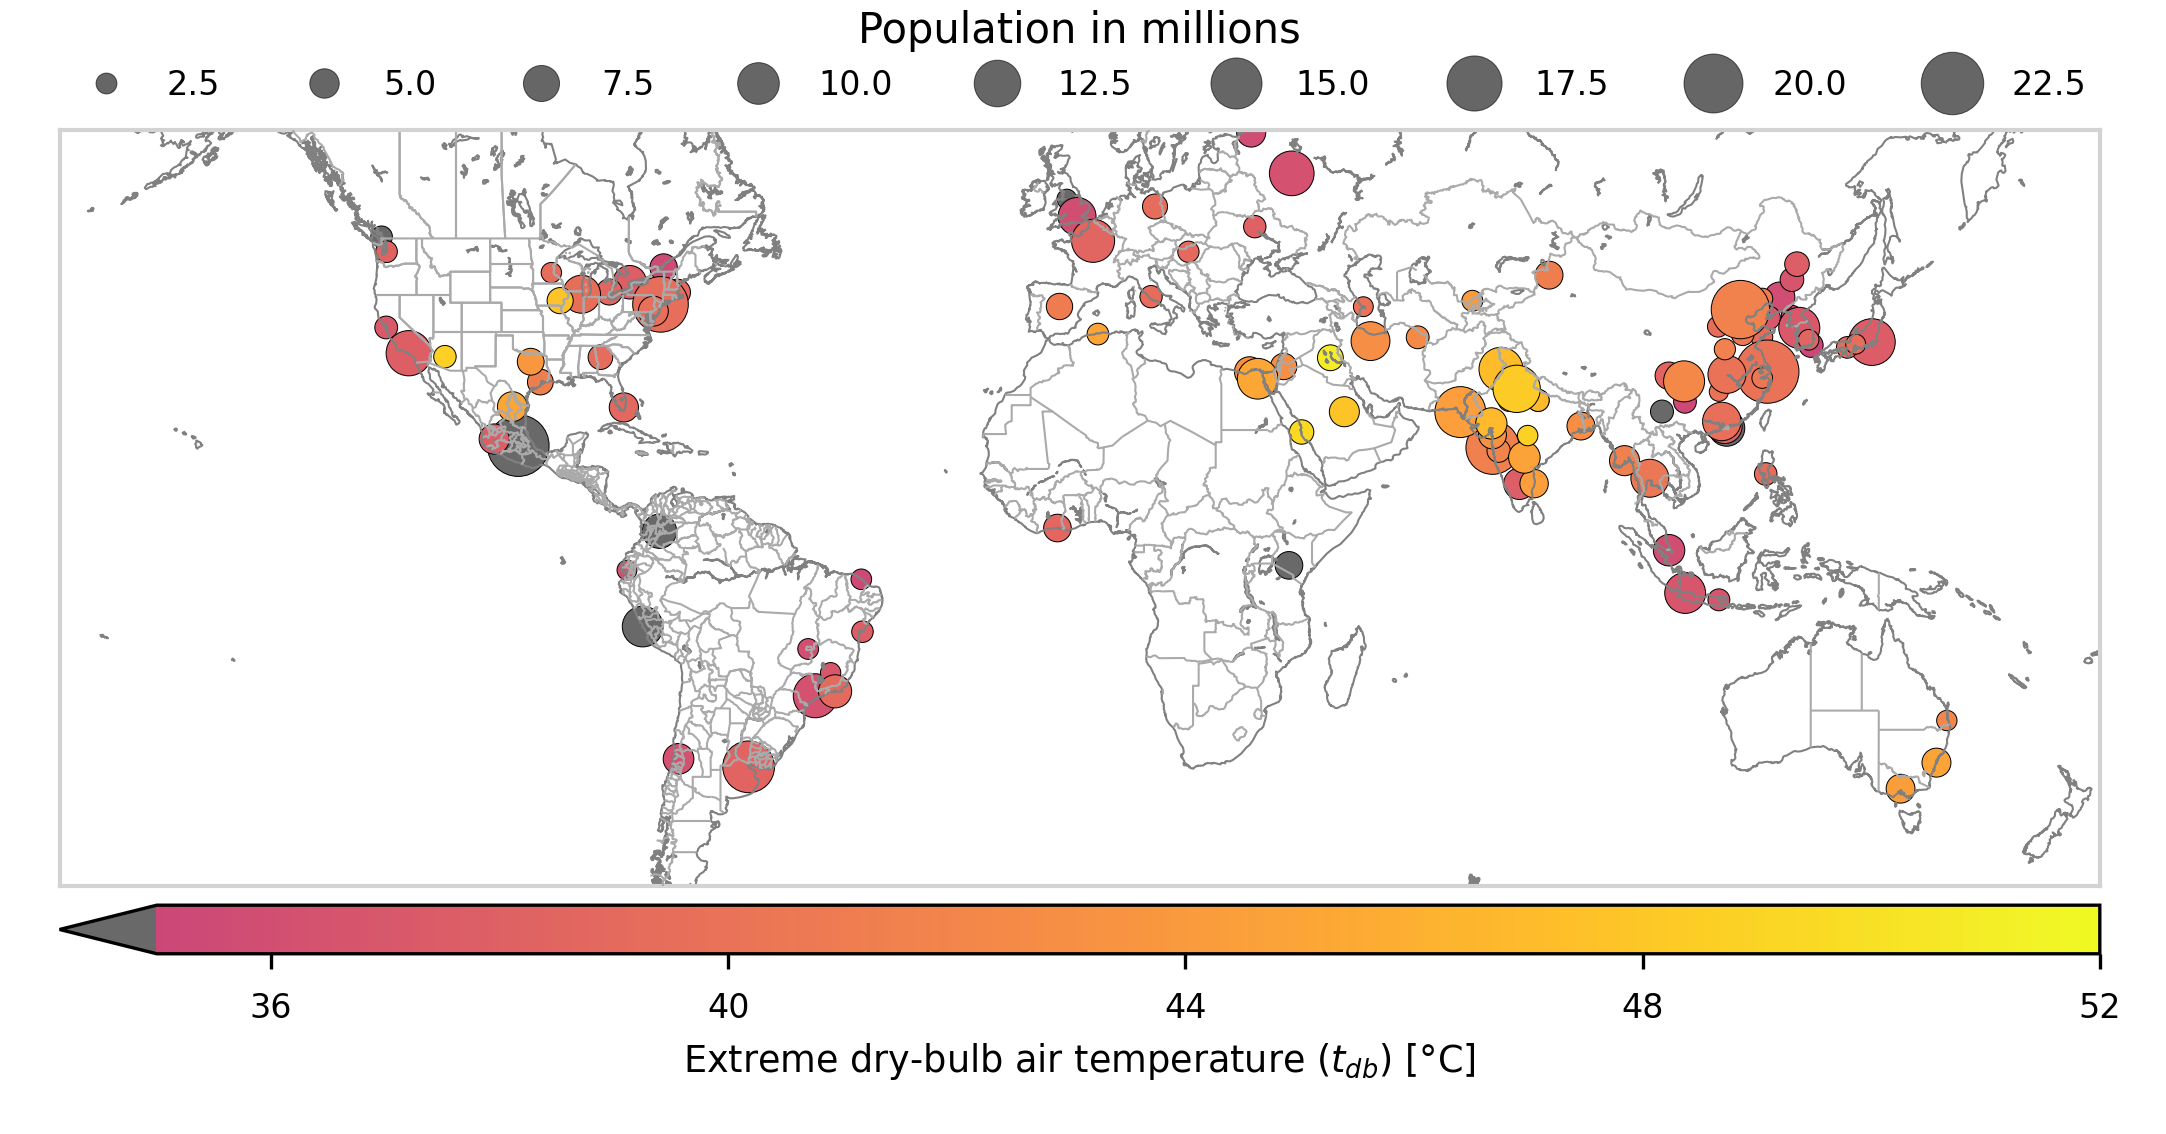
\includegraphics[width=\textwidth]{figures/map-population-temperature}
    \caption{Most populous 115 cities worldwide}
    \label{fig:map-population-temperature}
\end{figure*}

Each marker shows where the city is located, the dot size is proportional to the number of people living in that urban area, while the color shows the extreme \ac{t-db} recorded in that city.
In 2020, a total of approximately 650 million people (8~\% percent of the global population) lived in the urban agglomerate of the 115 largest cities.
In 95 of these cities, \ac{t-db} higher than 35~$^{\circ}$C\@ were recorded and their total population was approximately 550 million people.

We estimated that \var{cities_benefit_fan_08} of the most populous cities the use of electric fans that can generate \ac{v} up to 0.8~m/s would be beneficial.
The \mycite{GaggeSET} model predicted that healthy adults living in \var{cities_benefit_fan_02} cities (approximately \var{people_no_strain_still_air} million inhabitants) should not experience heat strain even without increasing air movement. 
However, they should still be encouraged in using electric fans to improve their thermal conditions in an energy-efficient way.
The model also predicts that \var{people_no_strain_v_08} million inhabitants would be better off using electric fans (\ac{v} up to 0.8~m/s) rather than not using them and they should not experience heat strain.

\begin{figure*}[thb!]
    \centering
    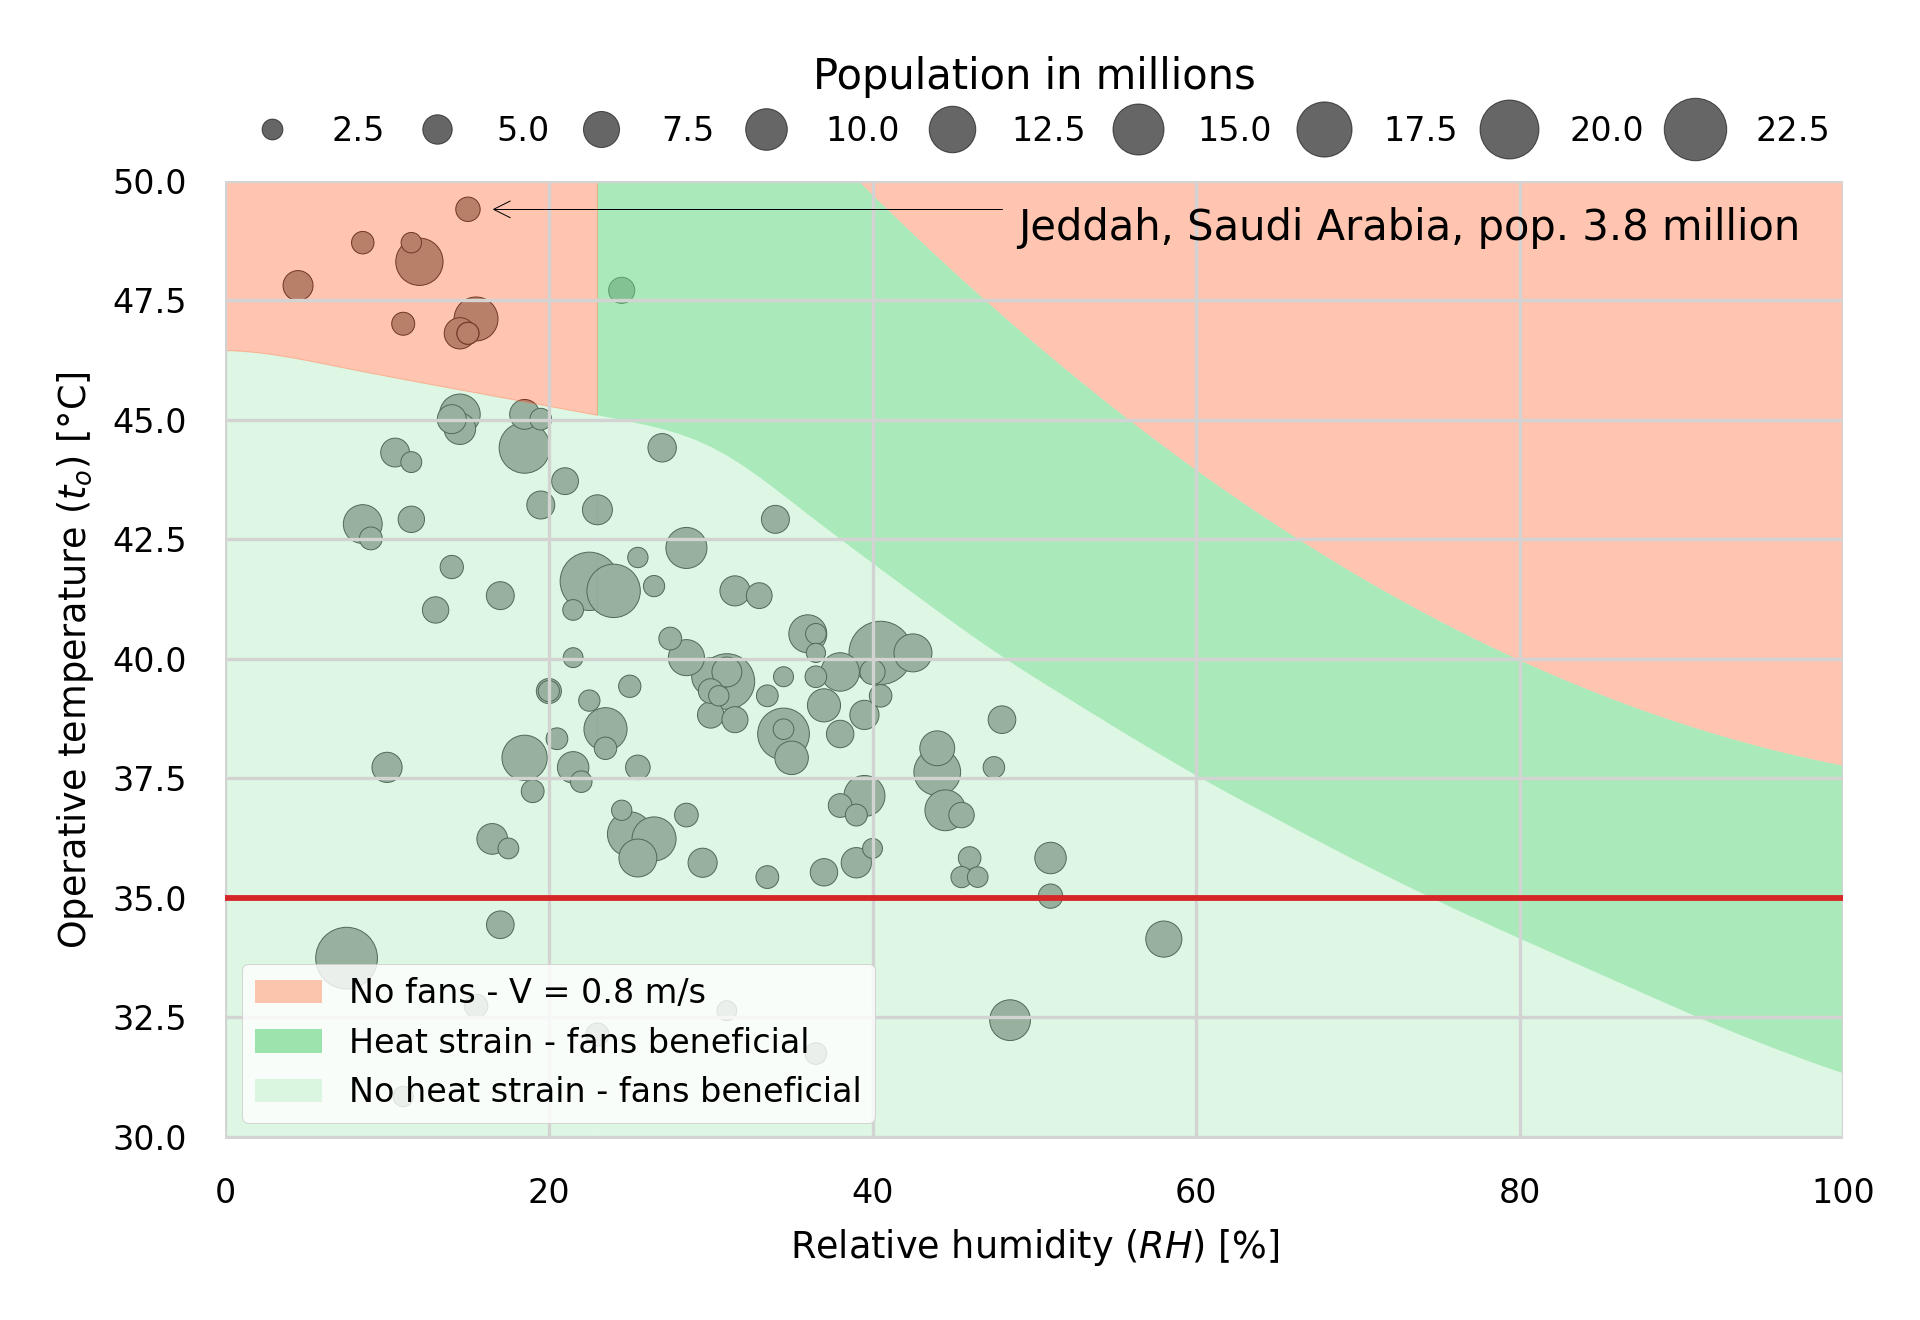
\includegraphics[width=\textwidth]{figures/use_fans_and_population}
    \caption{Environmental conditions under which the use of electric fans is beneficial, for more information on how to interpret the Figure please refer to the caption of Figure~\ref{fig:use_fans_experimental}.
    Each dot shows the maximum extreme climate conditions recorded over the last 20 years in each of the 115 most populous cities worldwide.}
    \label{fig:use_fans_and_population}
\end{figure*}

\subsection{Sweat Rate}\label{subsec:sweat-rate}

The predicted values of \ac{m-sweat} for \ac{v}~=~0.2~m/s at different combinations of \ac{t-db} and \ac{rh} are shown in Figure~\ref{fig:sweat_rate}A while the predicted differences in \ac{m-sweat} between \ac{v}~=~0.8~m/s and \ac{v}~=~0.2~m/s are shown in Figure~\ref{fig:sweat_rate}B\@.
In most of the combinations of \ac{t-db} and \ac{rh} the predicted values of \ac{m-sweat} are slightly higher in the `still air conditions' than when \ac{v}~=~0.8~m/s.
On the other hand, \ac{m-sweat} are higher with fan use when \ac{rh} is lower than 40~\% and \ac{t-db} higher than 40~$^{\circ}$C\@.
This can be explained by the fact that with low \ac{rh} and high \ac{t-db} almost all the sweat secreted on the skin surface would evaporate even without a fan, due to the high gradient in water vapour pressure between the skin and the air.
With elevated air speeds more sweat is needed to compensate for the additional sensible heat gains.
It should be noted, that in these conditions the maximum predicted difference in sweat losses due to fan use is always lower than 30 mL/h, a difference that could be compensated by the ingestion of approximately 1 glass (i.e., 250 mL) of water every 8 hours.

\begin{figure*}[thb!]
    \centering
    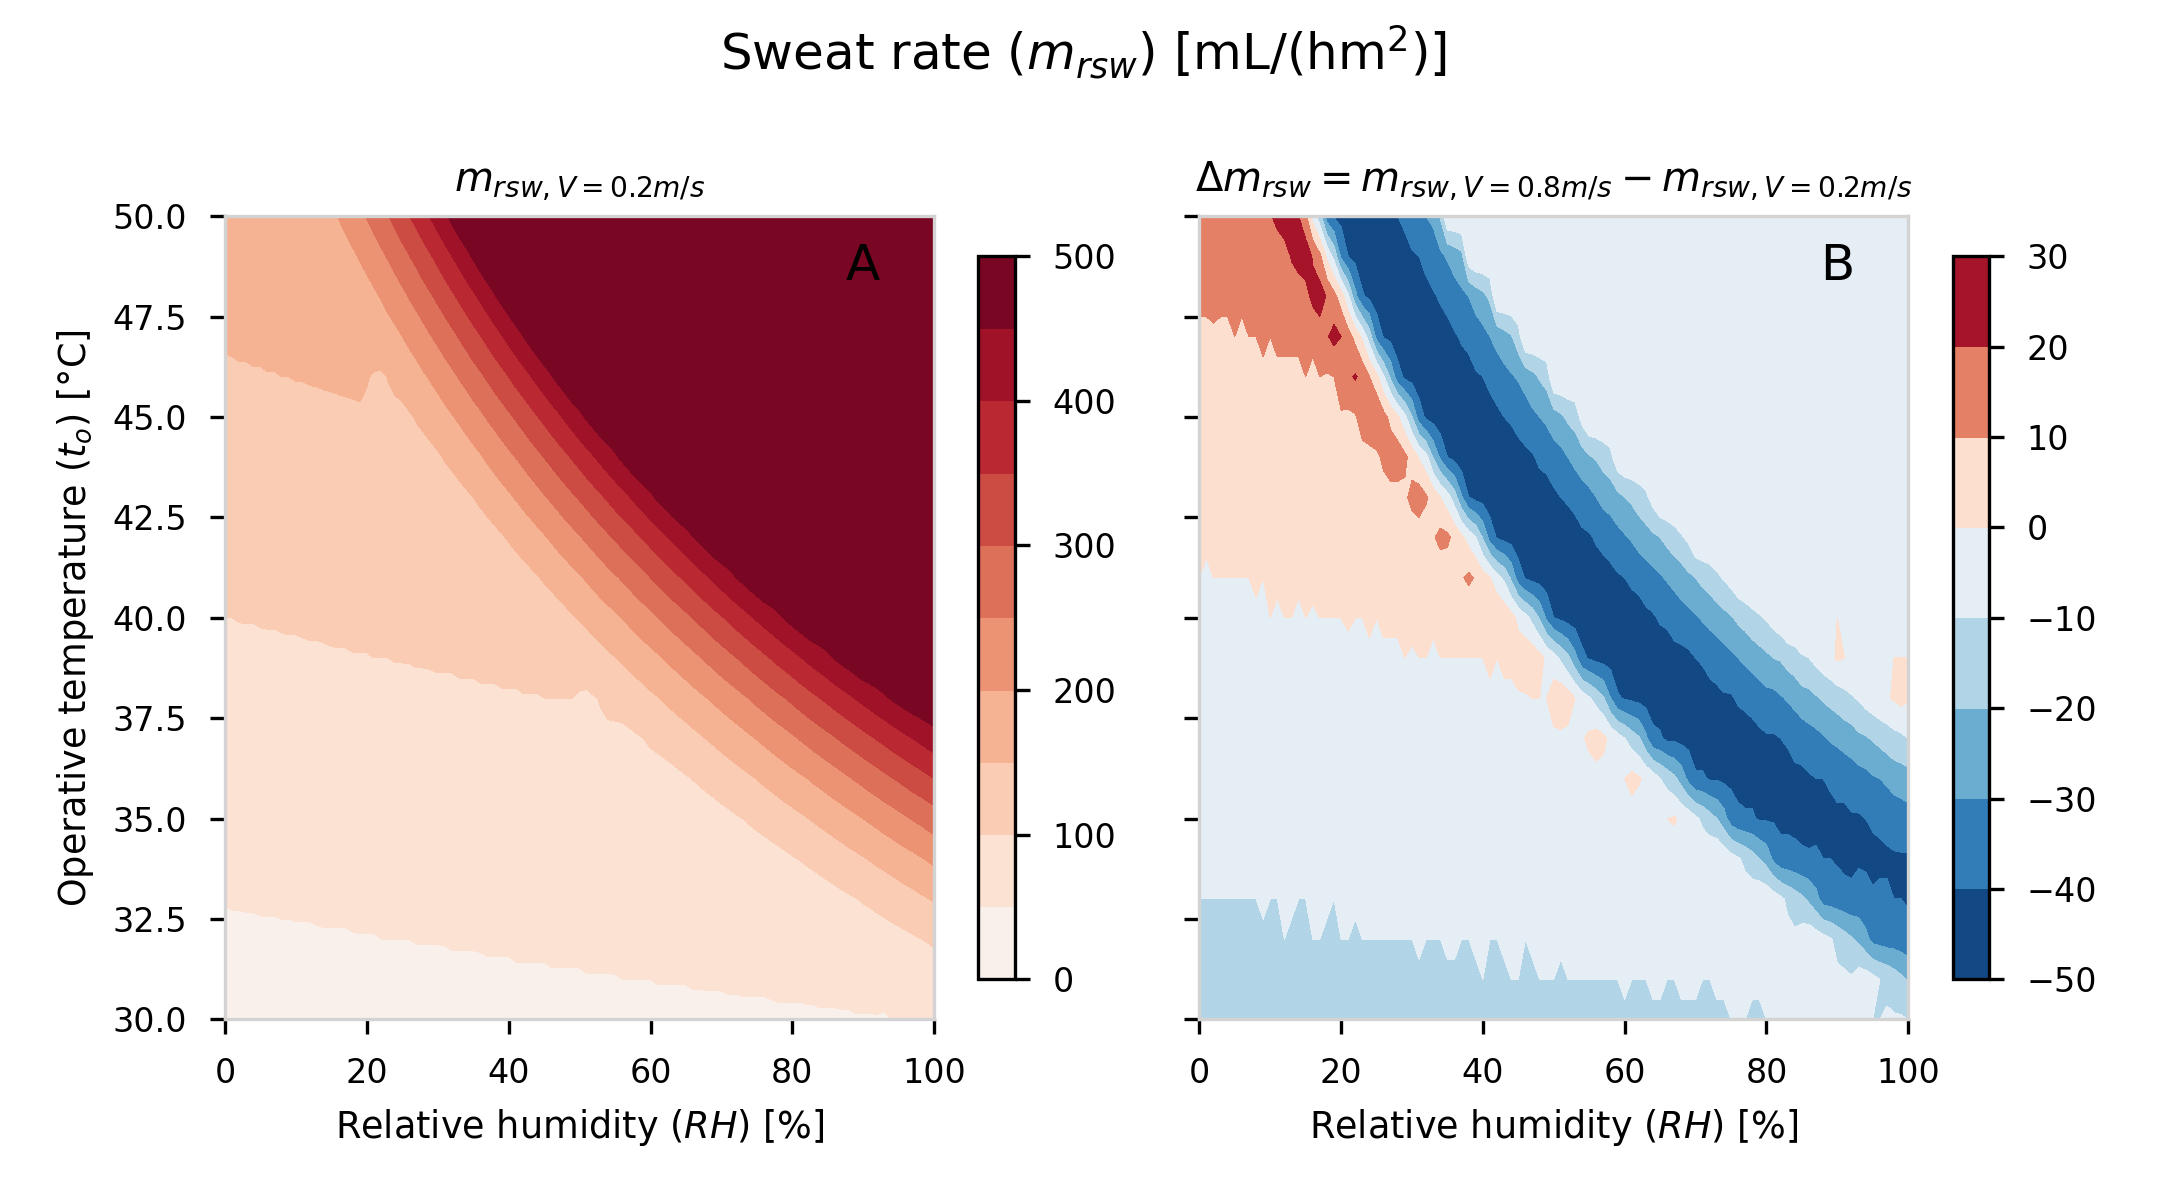
\includegraphics[width=\textwidth]{figures/sweat_rate}
    \caption{Predicted \acf{m-sweat} at different combinations of \acf{t-db} and \acf{rh} for two values \acf{v}~=~0.2~m/s and 0.8~m/s.}
    \label{fig:sweat_rate}
\end{figure*}

% note OJ Did you compare these estimated data to those reported in our physiological studies? Might be helpful